%%% Test a table
%
% Set the \input{} to the table you want to test, then typeset this file
%
\documentclass[12pt,twoside,a4paper]{book}
%\documentclass[draft,a4paper]{book}
%% use [showframe] to show the frames
\usepackage[showframe]{geometry}
\usepackage{longtable}% Allow for split of the table over more than one page
\usepackage{rotating} % Make it possible to rotate headers
\usepackage[normalsize]{caption} % Keep captions to (long)tables normal sized
% must go *after* rotating package
\usepackage{booktabs} % To get nice table layout
%
% To include graphics in tables
\usepackage{graphicx}
%
%% Settings from the main text we also need for the test
\usepackage{fontspec}
\setmainfont{Hoefler Text}[]
%\setmainfont{Times New Roman}[]
\newfontfamily\greekfont{Times New Roman}
\newfontfamily\hebrewfont{Arial Hebrew}
\newfontfamily\arabicfont{Arial Unicode MS}
\newfontfamily\astrofont{Menlo}
\newcommand\astro[1]{{\astrofont #1}}
%%
\usepackage[quiet]{polyglossia}
\setmainlanguage{latin}
\setotherlanguage{greek}
\setotherlanguage{hebrew}
\setotherlanguage{arabic}
%
\usepackage{lipsum} % Provide random filler Lore ipsum text
%%% Special command for roman numerals
%% Usage: \rnum{<roman numeral>}
%% Example: \rnum{mdclxviii}
\newcommand{\rnum}[1]{%
\textsc{#1}%
}
%
\begin{document}

%% Longtable version
%%%% Liber I p43
%%
%%% Count out columns for fixed-width source font
% 000000011111111112222222222333333333344444444445555555555666666666677777777778
% 345678901234567890123456789012345678901234567890123456789012345678901234567890
%
%%
\begin{tabnums} % Select monospaced numbers
%\tiny
%\scriptsize
\footnotesize
%\small
%\normalsize
%% Modify separation between columns
\setlength{\tabcolsep}{2.4pt}
%% Modify distance between rows
%\renewcommand{\arraystretch}{1.2}
%% Define reference symbols
\newcommand{\dg}{\scriptsize †}
\newcommand{\ddg}{\scriptsize ‡}
%% Local command to define small header
\newcommand{\sh}[1]{\multicolumn{1}{c}{\tiny{#1}}}
%% Names of the months, to save us a lot of typing
\newcommand{\rabx}{Rabie prior}
\newcommand{\rabz}{Rabie posterior}
\newcommand{\giux}{Giumadi prior}
\newcommand{\giuz}{Giumadi posterior}
\newcommand{\rege}{Regeb}
\newcommand{\saha}{Sahaben}
\newcommand{\rama}{Ramadhan}
\newcommand{\scew}{Scewal}
\newcommand{\dulk}{Dulkaidathi}
\newcommand{\dulc}{Dulchagiathi}
\newcommand{\muha}{Muharam}
\newcommand{\seph}{Sephar}
%% Let longtable process the whole table in one go
\setcounter{LTchunksize}{100}
\begin{longtable}[c]{@{}r  c  c  c  c  r@{~}l l l l l@{}}
\toprule
 & \multicolumn{9}{c}{\Large\textsc{Tabula periodi magnae Hagarenorum}}\\
\toprule
% Put a reference to the first page of the table in the List of Tables
% Tables in the LoT are listed on the 'section' level
% '\numberline{\thetable}' puts the number of the table before the
% title, correctly indented.
% '\protect' helps pass these commands without error.
\addcontentsline{lot}{section}{%
\protect\numberline{\thetable}Periodi magnae Hagarenorum}
\label{tab:p112}
%%
~ &
 \sh{Anni} &
 \sh{Cyclus} &
 \sh{Character} &
 \sh{Cyclus} \\
~ &
 \sh{periodi} &
 \sh{Lunae} &
 \sh{anni} &
 \sh{Solis} &
~ & & % 31 Martii
Periodus prima &
Periodus secunda &
Periodus tertia
\\
\midrule
\endfirsthead
\toprule
&
\multicolumn{9}{c}{\Large\textsc{Residuum tabulae periodi magnae Hagarenorum}}\\
\toprule
~ &
 \sh{Anni} &
 \sh{Cyclus} &
 \sh{Character} &
 \sh{Cyclus} \\
~ &
 \sh{periodi} &
 \sh{Lunae} &
 \sh{anni} &
 \sh{Solis} &
~ & & % 31 Martii
Periodus prima &
Periodus secunda &
Periodus tertia
\\
\midrule
\endhead
%\bottomrule
  \addlinespace
  & \multicolumn{6}{l}{\super † \textgreek{ἐμβολ.[?]}}
  & \multicolumn{3}{l}{\super ‡ \textgreek{ὑπερή.[?]}}
\endfoot
\bottomrule
  \addlinespace
  & \multicolumn{6}{l}{\super † \textgreek{ἐμβολ.[?]}}
  & \multicolumn{3}{l}{\super ‡ \textgreek{ὑπερή.[?]}} \\
  \addlinespace
  % Put the table nr and title below the table, without entry in the LoT
  \caption[]{Periodi magnae Hagarenorum}
\endlastfoot
  & ~1 & 14 & 1 & F   & 31&Martii & \seph & \giuz & \scew \\
  & ~2 & 15 & 5 & E   & 20&Martii & \seph & \giuz & \scew & \ddg\\
\dg  
  & ~3 & 16 & 3 & D C &  9&Martii & \seph & \giuz & \scew \\
  & ~4 & 17 & 2 & B   & 28&Martii & \rabx & \rege & \dulk \\
\cmidrule{2-10}
  & ~5 & 18 & 6 & A   & 17&Martii & \rabx & \rege & \dulk \\
\dg
  & ~6 & 19 & 3 & G   &  6&Martii & \rabx & \rege & \dulk \\
  & ~7 & ~1 & 2 & F E & 24&Martii & \rabz & \saha & \dulc \\
\dg
  & ~8 & ~2 & 6 & D   & 13&Martii & \rabz & \saha & \dulc \\
\cmidrule{2-10}
  & ~9 & ~3 & 5 & C   &  1&April. & \giux & \rama & \muha & \ddg\\
  & 10 & ~4 & 3 & B   & 22&Martii & \giux & \rama & \muha \\
\dg
  & 11 & ~5 & 7 & A G & 10&Martii & \giux & \rama & \muha \\
  & 12 & ~6 & 6 & F   & 29&Martii & \giuz & \scew & \seph \\
\cmidrule{2-10}
  & 13 & ~7 & 3 & E   & 18&Martii & \giuz & \scew & \seph & \ddg\\
\dg
  & 14 & ~8 & 1 & D   &  8&Martii & \giuz & \scew & \seph \\
  & 15 & ~9 & 7 & C B & 26&Martii & \rege & \dulk & \rabx \\
\dg
  & 16 & 10 & 4 & A   & 15&Martii & \rege & \dulk & \rabx \\
\cmidrule{2-10}
  & 17 & 11 & 3 & G   &  3&April. & \saha & \dulc & \rabz \\
  & 18 & 12 & 7 & F   & 23&Martii & \saha & \dulc & \rabz & \ddg\\
\dg
  & 19 & 13 & 5 & E D & 12&Martii & \saha & \dulc & \rabz \\
  & 20 & 14 & 4 & C   & 31&Martii & \rama & \muha & \giux \\
\cmidrule{2-10}
  & 21 & 15 & 4 & B   & 20&Martii & \rama & \muha & \giux \\
\dg
  & 22 & 16 & 1 & A   &  9&Martii & \rama & \muha & \giux \\
  & 23 & 17 & 5 & G F & 27&Martii & \scew & \seph & \giuz & \ddg\\
  & 24 & 18 & 4 & E   & 17&Martii & \scew & \seph & \giuz \\
\cmidrule{2-10}
\dg
  & 25 & 19 & 6 & D   &  6&Martii & \scew & \seph & \giuz \\
  & 26 & ~1 & 5 & C   & 25&Martii & \dulk & \rabx & \rege \\
\dg
  & 27 & ~2 & 2 & B A & 13&Martii & \dulk & \rabx & \rege \\
  & 28 & ~3 & 1 & G   &  1&April. & \dulc & \rabz & \saha \\
\cmidrule{2-10}
  & 29 & ~4 & 5 & F   & 21&Martii & \dulc & \rabz & \saha & \ddg\\
\dg
  & 30 & ~5 & 3 & E   & 11&Martii & \dulc & \rabz & \saha \\
  & 31 & ~6 & 2 & D C & 29&Martii & \muha & \giux & \rama \\
  & 32 & ~7 & 6 & B   & 18&Martii & \muha & \giux & \rama \\
\cmidrule{2-10}
\dg
  & 33 & ~8 & 3 & A   &  7&Martii & \muha & \giux & \rama \\
  & 34 & ~9 & 3 & G   & 27&Martii & \seph & \giuz & \scew & \ddg\\
\dg
  & 35 & 10 & 7 & F E & 15&Martii & \seph & \giuz & \scew \\
  & 36 & 11 & 6 & D   &  2&April. & \rabx & \rege & \dulk \\
\cmidrule{2-10}
  & 37 & 12 & 3 & C   & 23&Martii & \rabx & \rege & \dulk \\
\dg
  & 38 & 13 & 7 & B   & 12&Martii & \rabx & \rege & \dulk \\
  & 39 & 14 & 6 & A G & 30&Martii & \rabz & \saha & \dulc & \ddg\\
  & 40 & 15 & 4 & F   & 20&Martii & \rabz & \saha & \dulc \\
\cmidrule{2-10}
\dg
  & 41 & 16 & 1 & E   &  9&Martii & \rabz & \saha & \dulc \\
  & 42 & 17 & 7 & D   & 28&Martii & \giux & \rama & \muha \\
  & 43 & 18 & 4 & C B & 16&Martii & \giux & \rama & \muha & \ddg\\
\dg
  & 44 & 19 & 2 & A   &  6&Martii & \giux & \rama & \muha \\
\cmidrule{2-10}
  & 45 & ~1 & 1 & G   & 25&Martii & \giuz & \scew & \seph \\
\dg
  & 46 & ~2 & 5 & F   & 14&Martii & \giuz & \scew & \seph \\
  & 47 & ~3 & 4 & E D &  1&April. & \rege & \dulk & \rabx \\
  & 48 & ~4 & 1 & C   & 21&Martii & \rege & \dulk & \rabx \\
\cmidrule{2-10}
\dg
  & 49 & ~5 & 5 & B   & 10&Martii & \rege & \dulk & \rabx \\
  & 50 & ~6 & 4 & A   & 29&Martii & \saha & \dulc & \rabz & \ddg\\
  & 51 & ~7 & 2 & G F & 18&Martii & \saha & \dulc & \rabz \\
\dg
  & 52 & ~8 & 6 & E   &  7&Martii & \saha & \dulc & \rabz \\
\cmidrule{2-10}
  & 53 & ~9 & 5 & D   & 26&Martii & \rama & \muha & \giux \\
\dg
  & 54 & 10 & 2 & C   & 15&Martii & \rama & \muha & \giux \\
  & 55 & 11 & 1 & B A &  2&April. & \scew & \seph & \giuz & \ddg\\
  & 56 & 12 & 6 & G   & 23&Martii & \scew & \seph & \giuz \\
\cmidrule{2-10}
\dg
  & 57 & 13 & 3 & F   & 12&Martii & \scew & \seph & \giuz \\
  & 58 & 14 & 2 & E   & 31&Martii & \dulk & \rabx & \rege \\
  & 59 & 15 & 6 & D C & 19&Martii & \dulk & \rabx & \rege & \ddg\\
\dg
  & 60 & 16 & 4 & B   &  9&Martii & \dulk & \rabx & \rege \\
\cmidrule{2-10}
  & 61 & 17 & 3 & A   & 28&Martii & \dulc & \rabz & \saha \\
  & 62 & 18 & 7 & G   & 17&Martii & \dulc & \rabz & \saha \\
\dg
  & 63 & 19 & 4 & F E &  5&Martii & \dulc & \rabz & \saha \\
  & 64 & ~1 & 3 & D   & 24&Martii & \muha & \giux & \rama & \ddg\\
\cmidrule{2-10}
\dg
  & 65 & ~2 & 1 & C   & 14&Martii & \muha & \giux & \rama \\
  & 66 & ~3 & 7 & B   &  2&April. & \seph & \giuz & \scew \\
  & 67 & ~4 & 4 & A G & 21&Martii & \seph & \giuz & \scew \\
\dg
  & 68 & ~5 & 1 & F   & 10&Martii & \seph & \giuz & \scew \\
\cmidrule{2-10}
  & 69 & ~6 & 7 & E   & 29&Martii & \rabx & \rege & \dulk & \ddg\\
  & 70 & ~7 & 5 & D   & 18&Martii & \rabx & \rege & \dulk \\
\dg
  & 71 & ~8 & 2 & C B &  7&Martii & \rabx & \rege & \dulk \\
  & 72 & ~9 & 1 & A   & 26&Martii & \rabz & \saha & \dulc \\
\cmidrule{2-10}
\dg
  & 73 & 10 & 5 & G   & 15&Martii & \rabz & \saha & \dulc \\
  & 74 & 11 & 4 & F   &  3&April. & \giux & \rama & \muha \\
  & 75 & 12 & 1 & E D & 22&Martii & \giux & \rama & \muha \\
\dg
  & 76 & 13 & 5 & C   & 11&Martii & \giux & \rama & \muha & \ddg\\
\end{longtable}
\end{tabnums}

%% Regular table version

\lipsum[1]
\begin{table}[htbp]
  %% Tabula convertendi ostenta in sexagesimas et vice versa
%% Liber Primus, p.6, PDF 89
%%
%%% Count out columns for fixed-width source font
% 000000011111111112222222222333333333344444444445555555555666666666677777777778
% 345678901234567890123456789012345678901234567890123456789012345678901234567890
%
%% Select a general font size (uncomment one from the list)
%\tiny
%\scriptsize
%\footnotesize
%\small
\normalsize
%% Center the whole table left-right
\centering
%% Modify separation between columns
\setlength{\tabcolsep}{3pt}
%% Modify distance between rows
\renewcommand{\arraystretch}{1.1}
%% Define column header format
\newcommand{\colhead}[1]{\multicolumn{1}{c}{\footnotesize #1}}
%
\begin{tabular}{@{} r r r r  c r r r r }
\toprule
  \multicolumn{9}{c}{\Large\scshape Tabula convertendi ostenta} \\
  \multicolumn{9}{c}{\Large\scshape in sexagesimas et v.v.} \\
\toprule
  \multicolumn{4}{c}{\normalsize\scshape Ostenta in sexagesimas} & &
  \multicolumn{4}{c}{\normalsize\scshape Sexagesimas in ostenta}
\\
\cmidrule[\heavyrulewidth]{1-4} \cmidrule[\heavyrulewidth]{6-9}
\colhead{Ostenta} &
\colhead{Sexag.} &
\colhead{Sexag.} &
\colhead{Sexag.} &
\hspace{8mm} &
\colhead{Sexag.} &
\colhead{Sexag.} &
\colhead{Ostenta} &
\colhead{Ostenta}
\\
\cmidrule{1-4} \cmidrule{6-9}
   1 &  0' &  3'' & 20''' & &  0' &  1'' &    0' & 324'' \\
   2 &  0' &  6'' & 40''' & &  0' &  2'' &    0' & 648'' \\
   3 &  0' & 10'' &  0''' & &  0' &  3'' &    0' & 972'' \\
   4 &  0' & 13'' & 20''' & &  0' &  4'' &    1' & 210'' \\
   5 &  0' & 16'' & 40''' & &  0' &  5'' &    1' & 540'' \\
   6 &  0' & 20'' &  0''' & &  0' &  6'' &    1' & 864'' \\
   7 &  0' & 23'' & 20''' & &  0' &  7'' &    2' & 108'' \\
   8 &  0' & 26'' & 40''' & &  0' &  8'' &    2' & 432'' \\
   9 &  0' & 30'' &  0''' & &  0' &  9'' &    2' & 756'' \\
  10 &  0' & 33'' & 20''' & &  0' & 10'' &    3' &   0'' \\
  20 &  1' &  6'' & 40''' & &  0' & 20'' &    6' &   0'' \\
  30 &  1' & 40'' &  0''' & &  0' & 30'' &    9' &   0'' \\
  40 &  2' & 13'' & 20''' & &  0' & 40'' &   12' &   0'' \\
  50 &  2' & 46'' & 40''' & &  0' & 50'' &   15' &   0'' \\
  60 &  3' & 20'' &  0''' & &  1' & 60'' &   18' &   0'' \\
  70 &  3' & 53'' & 20''' & &  2' &  0'' &   36' &   0'' \\
  80 &  4' & 26'' & 40''' & &  3' &  0'' &   54' &   0'' \\
  90 &  5' &  0'' &  0''' & &  4' &  0'' &   72' &   0'' \\
 100 &  5' & 33'' & 20''' & &  5' &  0'' &   90' &   0'' \\
 200 & 11' &  6'' & 40''' & &  6' &  0'' &  108' &   0'' \\
 300 & 16' & 40'' &  0''' & &  7' &  0'' &  126' &   0'' \\
 400 & 22' & 13'' & 20''' & &  8' &  0'' &  144' &   0'' \\
 500 & 27' & 46'' & 40''' & &  9' &  0'' &  162' &   0'' \\
 600 & 33' & 20'' &  0''' & & 10' &  0'' &  180' &   0'' \\
 700 & 38' & 53'' & 20''' & & 20' &  0'' &  360' &   0'' \\
 800 & 44' & 26'' & 40''' & & 30' &  0'' &  540' &   0'' \\
 900 & 50' &  0'' &  0''' & & 40' &  0'' &  720' &   0'' \\
1000 & 55' & 33'' & 20''' & & 50' &  0'' &  900' &   0'' \\
\multicolumn{4}{c}{}      & & 60' &  0'' & 1080' &   0'' \\
\bottomrule
\end{tabular}
%
\caption{Convertendi ostenta in sexagesimas et vice versa}
\label{tab:p006}
%

\end{table}

\lipsum[4]
\begin{table}[htbp]
  %% Dies Hebdomadis
%% Liber Primus, p.8, PDF 91
%%
%%% Count out columns for fixed-width source font
% 000000011111111112222222222333333333344444444445555555555666666666677777777778
% 345678901234567890123456789012345678901234567890123456789012345678901234567890
%
%% Select a general font size (uncomment one from the list)
%\tiny
%\scriptsize
%\footnotesize
%\small
\normalsize
%% Center the whole table left-right
\centering
%% Modify separation between columns
%\setlength{\tabcolsep}{0.5em}
%% Modify distance between rows
%\renewcommand{\arraystretch}{0.85}
%%
\begin{tabular}{@{} r r r  r l @{}}
\multicolumn{3}{c}{Dies hebdomadis Persicae} &
\multicolumn{2}{c}{\textsc{Aliter Persice}}
\\
\cmidrule(lr){1-3} \cmidrule(lr){4-5}
\texthebrew{ שנבה}[?] % some random characters as filler text
% from https://en.wikibooks.org/wiki/Persian/Phrasebook/Days_of_the_Week
% and persian wikipedia page for 'names of the days of the week'
% (rightmost column)
& \textarabic{یک‌شنبه}[?] % yekšanbe
& \textarabic{ل}[?]
& 1
& \textit{Ruz iache}
\\
\texthebrew{דושנבה}[?] % došanbe
& \textarabic{دوشنبه}[?]
& \textarabic{ب}[?]
& 2
& \textit{Ruz duiemi}
\\
\texthebrew{סהשׁנבה‎}[?] % sešanbe
& \textarabic{سه‌شنبه}[?]
& \textarabic{ج}[?]
& 3
& \textit{Ruz siumi}
\\
\texthebrew{גה‎ שנבה}[?] % chahâršanbe
& \textarabic{چهارشنبه}[?]
& \textarabic{ﺩ}[?]
& 4
& \textit{Ruz tzeharmi}
\\
\texthebrew{שנבה}[?] % panjšanbe
& \textarabic{پنج‌شنبه}[?]
& \textarabic{م}[?]
& 5
& \textit{Ruz pengemin}
\\
\texthebrew{אדיבה}[?] % jom'e
& \textarabic{آدینه}[?]
& \textarabic{و}[?]
& 6
& \textit{Ruz schesmin}
\\
\texthebrew{שנבה}[?] % šanbe
& \textarabic{شنبه}[?]
& \textarabic{ز}[?]
& 7
& \textit{Ruz haphthemi}
\\
\addlinespace
\addlinespace
\end{tabular}


\begin{tabular}{@{} r r   r r c @{}}
\multicolumn{2}{c}{Turciae hebdomadis dies} &
\multicolumn{3}{c}{Secundum planetas}
\\
\cmidrule(lr){1-2} \cmidrule(lr){3-5}
\texthebrew{גםעה}[?]
& \textarabic{[Arabic]}[?]
& \texthebrew{רח ותל}[?]
& \textarabic{زحل}[?]
& \astro{♄}
\\
\texthebrew{נםצה ארתםי}[?]
& \textarabic{[Arabic]}[?]
& \texthebrew{רח םשתרי}[?]
& \textarabic{المشتري}[?]
& \astro{♃}
\\
\texthebrew{בור בוה}[?]
& \textarabic{[Arabic]}[?]
& \texthebrew{רח םריח}[?]
& \textarabic{المريخ}[?]
& \astro{♂}
\\
\texthebrew{בור ארתםי}[?]
& \textarabic{[Arabic]}[?]
& \texthebrew{רח אפמאב}[?]
& \textarabic{الأرض}[?]
& \astro{☉}
\\
\texthebrew{צלי}[?]
& \textarabic{[Arabic]}[?]
& \texthebrew{רח והר}[?]
& \textarabic{الزهرة}[?]
& \astro{♀}
\\
\texthebrew{גהר שגבה}[?]
& \textarabic{[Arabic]}[?]
& \texthebrew{רח צטראר}[?]
& \textarabic{عطارد}[?]
& \astro{☿}
\\
\texthebrew{בגג שגבה}[?]
& \textarabic{[Arabic]}[?]
& \texthebrew{רחםה}[?]
& \textarabic{[Arabic]}[?]
& \astro{☾}
\end{tabular}
%
\caption{Dies Hebdomadis}
\label{tab:p008}

\end{table}

\lipsum[5]
\begin{table}[htbp]
  %% Version of novilunia table in vertical style, like the original
%% Liber Primus, p.27, PDF 110
%%
%% requires \usepackage{rotating}
%\begin{table}[htbp]
%\centering
\begin{tabular}{| r | r | r | r | r |}
\hline
\begin{sideways}
Linea: mensium
\end{sideways}
&
\begin{sideways}
Annus primus
\end{sideways}
&
\begin{sideways}
Annus secundus
\end{sideways}
&
\begin{sideways}
Annus tertius
\end{sideways}
&
\begin{sideways}
Annus quartus
\end{sideways}
\\
\hline
  1 & 1    & 23 & 15 & 7
\\ \cline{2-5}
  2 & 1.30 & 22 & 14 & 6
\\ \cline{2-5}
  3 & 30   & 22 & 14 & 6
\\ \cline{2-5}
  4 & 29   & 21 & 13 & 5
\\ \cline{2-5}
  5 & 29   & 21 & 13 & 5
\\ \cline{2-5}
  6 & 28   & 20 & 12 & 4
\\ \cline{2-5}
  7 & 28   & 20 & 12 & 4
\\ \cline{2-5}
  8 & 27   & 19 & 11 & 3
\\ \cline{2-5}
  9 & 27   & 19 & 11 & 3
\\ \cline{2-5}
 10 & 26   & 18 & 10 & 2
\\ \cline{2-5}
 11 & 26   & 18 & 10 & 2
\\ \cline{2-5}
 12 & 25   & 17 &  9 & 2
\\
\hline
\end{tabular}
%\caption{Novilunia in mensibus Tetraetirides Graecae}
%\label{tab:novilunia}
%\end{table}

\end{table}

\lipsum[6]
\begin{table}[htbp]
  % Version of novilunia table with horizontal layout
%% Liber Primus, p.27, PDF 110
%%
%%% Count out columns for fixed-width source font
% 000000011111111112222222222333333333344444444445555555555666666666677777777778
% 345678901234567890123456789012345678901234567890123456789012345678901234567890
%
{
\tabnums % Select monospaced numbers
%% Select a general font size (uncomment one from the list)
%\tiny
%\scriptsize
%\footnotesize
%\small
\normalsize
%% Center the whole table left-right
\centering
%% Modify separation between columns
%\setlength{\tabcolsep}{0.5em}
%% Modify distance between rows
%\renewcommand{\arraystretch}{0.85}
%%
\begin{tabular}{@{} l *{12}{r} @{}}
\toprule
\multicolumn{13}{ c }{\Large\textsc{Novilunia in mensibus}} \\
\multicolumn{13}{ c }{\Large\textsc{Tetraeteridis Graecae}} \\
\toprule
~ &
\multicolumn{12}{ c }{Mensium}
\\
\cmidrule(l){2-13}
Annus &
1 & 2 & 3 & 4 & 5 & 6 & 7 & 8 & 9 & 10 & 11 & 12
\\
\midrule
Primus &
1 & 1\altsep{}30
        & 30 & 29 & 29 & 28 & 28 & 27 & 27 & 26 & 26 & 25 
\\
Secundus &
23 & 22 & 22 &21  &21  & 20 & 20 & 19 & 19 & 18 & 18 & 17
\\
Tertius &
15 & 14 & 14 & 13 & 13 & 12 & 12 & 11 & 11 & 10 & 10 & 9
\\
Quartus &
7 & 6 & 6 & 5 & 5 & 4 & 4 & 3 & 3 & 2 & 2 & 2
\\
\bottomrule
\end{tabular}
%
\caption{Novilunia in mensibus Tetraetirides Graecae}
\label{tab:p027}
}

\end{table}

\lipsum[7]
\begin{table}[htbp]
  %%% Laterculum mensium Atticorum secundam anni quadrantes
%%% Liber I p33
%%
%% Table more horizontally spread out to make it look better without
%% text wrapping.
%
%% Names copied from Wikipedia: Attic calendar
%% then modified to match the original
%% - declension of quarter names θέρος -> θΕΡΙΝΟΙ
%% - no accents on the capitals
%% - Autumn: Φθινόπωρον -> ΟΠΩΡΙΝΟΙ
%% - Μουνιχιών -> Μουνυχιών (ι -> υ)
%% - Σκιροφοριών -> Σκιῤῥροφοριών (double ρ)
%% Added numbers to ensure the reader knows the order of the months
%%
%%% Count out columns for fixed-width source font
% 000000011111111112222222222333333333344444444445555555555666666666677777777778
% 345678901234567890123456789012345678901234567890123456789012345678901234567890
%
%% Select a general font size (uncomment one from the list)
%\tiny
%\scriptsize
%\footnotesize
%\small
\normalsize
%% Center the whole table left-right
\centering
%% Modify separation between columns
%\setlength{\tabcolsep}{0.5em}
%% Modify distance between rows
%\renewcommand{\arraystretch}{0.85}
%%
%% Four columns, one for each season
\begin{tabular}{@{}llll@{}}
\toprule
\multicolumn{4}{ c }{\Large\textsc{Laterculum mensium Atticorum}} \\
\multicolumn{4}{ c }{\Large\textsc{secundam anni quadrantes}} \\
\toprule
  \textgreek{Θερινοι}[?] & % Are the tonoi correct?
  \textgreek{Οπωρινοι}[?] &
  \textgreek{Χειμερινοι}[?] &
  \textgreek{Εαρινοι}[?]
\\
  \textgreek{μηνες}[?] &
  \textgreek{μηνες}[?] &
  \textgreek{μηνες}[?] &
  \textgreek{μηνες}[?]
\\
\midrule
%%
  \textgreek{Εκατομβαιών} &
  \textgreek{Πυανεψιών} &
  \textgreek{Γαμηλιών} &
  \textgreek{Μουνυχιών}
\\
  \textgreek{Μεταγειτνιών} &
  \textgreek{Μαιμακτηριών} &
  \textgreek{Ανθεστηριών} &
  \textgreek{Θαργηλιών}
\\
  \textgreek{Βοηδρομιών} &
  \textgreek{Ποσειδεών} &
  \textgreek{Ελαφηβολιών} &
  \textgreek{Σκιῤῥοφοριών}
\\
\bottomrule
\end{tabular}
%
\caption{Laterculum mensium Atticorum secundam anni quadrantes}
\label{tab:p033}

\end{table}

\lipsum[8]
\begin{table}[htbp]
  %%% Liber I p34
%%
%%% Count out columns for fixed-width source font
% 000000011111111112222222222333333333344444444445555555555666666666677777777778
% 345678901234567890123456789012345678901234567890123456789012345678901234567890
%
%% Select a general font size (uncomment one from the list)
%\tiny
%\scriptsize
%\footnotesize
%\small
\normalsize
%% Center the whole table left-right
\centering
%% Modify separation between columns
%\setlength{\tabcolsep}{0.5em}
%% Modify distance between rows
%\renewcommand{\arraystretch}{0.85}
%%
\begin{tabular}{@{}rrrrrl@{}}
\toprule
\multicolumn{6}{ c }{\Large\textsc{Laterculum neomeniarum}} \\
\multicolumn{6}{ c }{\large\textsc{lunarium in mensibus Atticis}} \\
\toprule
 1 & 1.   & 23 & 15 & 7 &\textgreek{ἐκατομβαιών} \\
 2 & 1\slash{}30 & 22 & 14 & 6 &\textgreek{μεταγειτνιών} \\
 3 & 30   & 22 & 14 & 6 &\textgreek{βοηδρομιών} \\
 4 & 29   & 21 & 13 & 5 &\textgreek{πυανεψιών} \\
 5 & 29   & 21 & 13 & 5 &\textgreek{μαιμακτηριών} \\
 6 & 28   & 20 & 12 & 4 &\textgreek{ποσειδεών} \\
 7 & 26   & 18 & 10 & 3 &\textgreek{υαμηλιών} \\
 8 & 25   & 17 &  9 & 3 &\textgreek{ανθεστηριών} \\
 9 & 25   & 17 &  9 & 2 &\textgreek{ἐλαφηβολιών} \\
10 & 24   & 16 &  8 & 2 &\textgreek{μουνυχιών} \\
11 & 24   & 16 &  8 & 1 &\textgreek{θαργηλιών} \\
12 & 23   & 15 &  7 & 1 &\textgreek{σκιῤῥοφοριών} \\
\bottomrule
\end{tabular}
%
\caption{Laterculum neomeniarum lunarium in mensibus Atticis}
\label{tab:p034}
%

\end{table}

\lipsum[9]
\begin{table}[htbp]
  %%% Liber I p38
%%
%%% Count out columns for fixed-width source font
% 000000011111111112222222222333333333344444444445555555555666666666677777777778
% 345678901234567890123456789012345678901234567890123456789012345678901234567890
%
\begin{tabnums} % Select monospaced numbers
%% Select a general font size (uncomment one from the list)
%\tiny
%\scriptsize
\footnotesize
%\small
%\normalsize
%% Center the whole table left-right
\centering
%% Modify separation between columns
%\setlength{\tabcolsep}{0.5em}
%% Modify distance between rows
\renewcommand{\arraystretch}{0.85}
%
%% Different daggers
\newcommand{\dsize}{\scriptsize}
\newcommand{\dc}{{\dsize †}}
\newcommand{\da}{{\dsize ‡}}
\newcommand{\db}{{◊}}
%% The angle with which to slant
\newcommand{\ang}{60}
%% Text size of the headers
\newcommand{\hdsize}{\scriptsize}
%% Define the column headers so both sub-tables are the same
\newcommand{\hdr}{%
\begin{tabular}[t]{r rrr r@{~}l r l}
~ &
\multicolumn{1}{c}{\begin{rotate}{\ang}\hdsize Anni periodi\end{rotate}} &
\multicolumn{1}{c}{\begin{rotate}{\ang}\hdsize Cyclus Lunnae\end{rotate}} &
\multicolumn{1}{c}{\begin{rotate}{\ang}\hdsize Dies collecti\end{rotate}} &
\multicolumn{2}{c}{\begin{rotate}{\ang}\hdsize
  \parbox[t]{3.5cm}{Neomenia\\\hspace*{5pt}1. mensis}
\end{rotate}} &
\multicolumn{2}{l}{\begin{turn}{\ang}\hdsize \textgreek{περιτταὶ ἡμέραι}\end{turn}}
}
%%
% Implemented as two subtables side-by-side
\begin{tabular}{@{}lc@{}}
\toprule
\multicolumn{2}{ c }{\Large\textsc{Tabula neomeniarum primi mensis}} \\
\multicolumn{2}{ c }{\large\textsc{Elidensis in annis periodi Olympicae}} \\
\toprule
% Left subtable
\hdr % tabular command and column headers
\\
\cmidrule{2-7}
  ~ &  1 &  5 &  392 &  9&Iulii & 0 & \dc \\
  ~ &  2 &  6 &  754 &  5&Aug. & 27 & \\
  ~ &  3 &  7 & 1116 &  2&Aug. & 24 & \\
\db &  4 &  8 & 1476 & 29&Iul. & 20 \\
\cmidrule{2-7}
  ~ &  5 &  9 & 1838 & 24&Iul. & 15 \\
  ~ &  6 & 10 & 2200 & 21&Iul. & 12 \\
  ~ &  7 & 11 & 2562 & 18&Iul. &  9 \\
\da &  8 & 12 & 2923 & 14&Iul. &  5 \\
\cmidrule{2-7}
  ~ &  9 & 13 & 3315 & 10&Iul. &  1 & \dc \\
  ~ & 10 & 14 & 3677 &  6&Aug. & 28 \\
  ~ & 11 & 15 & 4039 &  3&Aug. & 25 \\
\da & 12 & 16 & 4400 & 30&Iul. & 21 \\
\cmidrule{2-7}
  ~ & 13 & 17 & 4702 & 26&Iul. & 17 \\
  ~ & 14 & 18 & 5124 & 23&Iul. & 14 \\
  ~ & 15 & 19 & 5480 & 20&Iul. & 11 \\
\da & 16 &  1 & 5846 & 16&Iul. &  7 \\
\cmidrule{2-7}
  ~ & 17 &  2 & 6208 & 12&Iul. &  3 \\
  ~ & 18 &  3 & 6600 &  9&Iul. &  0 & \dc \\
  ~ & 19 &  4 & 6962 &  5&Aug. & 27 \\
\db & 20 &  5 & 7322 &  1&Aug. & 23 \\
\cmidrule{2-7}
  ~ & 21 &  6 & 7686 & 27&Iul. & 18 \\
  ~ & 22 &  7 & 8047 & 24&Iul. & 15 \\
  ~ & 23 &  8 & 8409 & 21&Iul. & 12 \\
\da & 24 &  9 & 8770 & 17&Iul. &  8 \\
\cmidrule{2-7}
  ~ & 25 & 10 &  9133 & 13&Iul. &  4 \\
  ~ & 26 & 11 &  9524 & 10&Iul. &  1 & \dc  \\
  ~ & 27 & 12 &  9886 &  6&Aug. & 28 \\
\da & 28 & 13 & 10247 &  2&Aug. & 24 \\
\cmidrule{2-7}
  ~ & 29 & 14 & 10609 & 29&Iul. & 20 \\
  ~ & 30 & 15 & 10971 & 26&Iul. & 17 \\
  ~ & 31 & 16 & 11333 & 23&Iul. & 14 \\
\da & 32 & 17 & 11694 & 19&Iul. & 10 \\
\cmidrule{2-7}
  ~ & 33 & 18 & 12056 & 29&Iul. &  6 \\
  ~ & 34 & 19 & 12418 & 26&Iul. &  3 \\
  ~ & 35 &  1 & 12810 & 23&Iul. &  0 & \dc  \\
\da & 36 &  2 & 13171 & 19&Aug. & 26 \\
\cmidrule{2-7}
  ~ & 37 &  3 & 13533 & 31&Iul. & 22 \\
  ~ & 38 &  4 & 13895 & 28&Iul. & 19 \\
  ~ & 39 &  5 & 14257 & 25&Iul. & 16 \\
\db & 40 &  6 & 14617 & 21&Iul. & 12 \\
\cmidrule{2-7}
\end{tabular}
%% next column
&
%%
% Right subtable
\hdr % tabular command and column headers
\\
\cmidrule{2-7}
  ~ & 41 &  7 & 14979 & 16&Iul. &  7 \\
  ~ & 42 &  8 & 15341 & 13&Iul. &  4 \\
  ~ & 43 &  9 & 15733 & 10&Iul. &  1 & \dc  \\
\da & 44 & 10 & 16094 &  5&Aug. & 27 \\
\cmidrule{2-7}
  ~ & 45 & 11 & 16456 &  1&Aug. & 23 \\
  ~ & 46 & 12 & 16818 & 29&Iul. & 20 \\
  ~ & 47 & 13 & 17180 & 26&Iul. & 27 \\
\da & 48 & 14 & 17541 & 22&Iul. & 13 \\
\cmidrule{2-7}
  ~ & 49 & 15 & 17903 & 18&Iul. &  9 \\
  ~ & 50 & 16 & 18265 & 15&Iul. &  6 \\
  ~ & 51 & 17 & 18627 & 12&Iul. &  3 & \dc  \\
\da & 52 & 18 & 19017 &  7&Aug. & 29 \\
\cmidrule{2-7}
  ~ & 53 & 19 & 19379 &  3&Aug. & 25 \\
  ~ & 54 &  1 & 19741 & 31&Iul. & 22 \\
  ~ & 55 &  2 & 20103 & 28&Iul. & 19 \\
\da & 56 &  3 & 20464 & 24&Iul. & 14 \\
\cmidrule{2-7}
  ~ & 57 &  4 & 20826 & 20&Iul. & 11 \\
  ~ & 58 &  5 & 21188 & 17&Iul. &  8 \\
  ~ & 59 &  6 & 21550 & 14&Iul. &  5 \\
\db & 60 &  7 & 21940 & 10&Iul. &  1 & \dc  \\
\cmidrule{2-7}
  ~ & 61 &  8 & 22302 &  4&Aug. & 26 \\
  ~ & 62 &  9 & 22664 &  1&Aug. & 23 \\
  ~ & 63 & 10 & 23026 & 29&Iul. & 20 \\
\da & 64 & 11 & 23388 & 25&Iul. & 16 \\
\cmidrule{2-7}
  ~ & 65 & 12 & 23750 & 21&Iul. & 12 \\
  ~ & 66 & 13 & 24112 & 18&Iul. &  9 \\
  ~ & 67 & 14 & 24474 & 15&Iul. &  6 \\
\da & 68 & 15 & 24865 & 11&Iul. &  2 & \dc  \\
\cmidrule{2-7}
  ~ & 69 & 16 & 25227 &  6&Aug. & 28 \\
  ~ & 70 & 17 & 25589 &  3&Aug. & 25 \\
  ~ & 71 & 18 & 25951 & 31&Iul. & 22 \\
\da & 72 & 19 & 26312 & 27&Iul. & 18 \\
\cmidrule{2-7}
  ~ & 73 &  1 & 26674 & 23&Iul. & 14 \\
  ~ & 74 &  2 & 27036 & 20&Iul. & 11 \\
  ~ & 75 &  3 & 27398 & 17&Iul. &  8 \\
\da & 76 &  4 & 27759 & 13&Iul. &  4 \\
\cmidrule{2-7}
\\
~ & \multicolumn{5}{l}{\super\dc{} \textgreek{ἐμβολ.}}\\
~ & \multicolumn{5}{l}{\super\da{} \textgreek{ἐξαιρ.}}\\
~ & \multicolumn{5}{l}{\super\db{} \textgreek{δισεξαιρεσιμαῖος [?]}}\\
\end{tabular}
\end{tabular}
%
\caption{Neomeniarum primi mensis Elidensis in annis periodi Olympicae}
\label{tab:p038}
\end{tabnums}

\end{table}

\lipsum[10]
\begin{table}[htbp]
  %%% Liber I p43
%%
%%% Count out columns for fixed-width source font
% 000000011111111112222222222333333333344444444445555555555666666666677777777778
% 345678901234567890123456789012345678901234567890123456789012345678901234567890
%
\begingroup
%% Select a general font size (uncomment one from the list)
%\tiny
\scriptsize
%\footnotesize
%\small
%\normalsize
%% Center the whole table left-right
\centering
%% Modify separation between columns
\setlength{\tabcolsep}{1.6pt}
%% Modify distance between rows
\renewcommand{\arraystretch}{1.2}
%
%% Define reference symbols
\newcommand{\da}{{\tiny †}}
\newcommand{\db}{{\tiny ‡}}
%% The angle with which to slant
\newcommand{\ang}{60}
%% Generate the column headers
\newcommand{\hdrs}{%
% A \multicolumn{} here would clash with \addcontentsline{}
\begin{rotate}{\ang}Anni periodi\end{rotate} &
&
\multicolumn{1}{c}{\begin{rotate}{\ang}\textgreek{Εκατομβαιών}\end{rotate}} & &
\multicolumn{1}{c}{\begin{rotate}{\ang}\textgreek{Μεταγειτνιών}\end{rotate}} & &
\multicolumn{1}{c}{\begin{rotate}{\ang}\textgreek{Βοηδρομιών}\end{rotate}} & &

\multicolumn{1}{c}{\begin{rotate}{\ang}\textgreek{Πυανεψιών}\end{rotate}} & &
\multicolumn{1}{c}{\begin{rotate}{\ang}\textgreek{Μαιμακτηριών}\end{rotate}} & &
\multicolumn{1}{c}{%
\begin{rotate}{\ang}\textgreek{Ποσειδεών \gnums{1}{α}}\end{rotate}} & &

\multicolumn{1}{c}{%
\begin{rotate}{\ang}\textgreek{Ποσειδεών \gnums{1}{β}}\end{rotate}} & &

\multicolumn{1}{c}{\begin{rotate}{\ang}\textgreek{Γαμηλιών}\end{rotate}} & &
\multicolumn{1}{c}{\begin{rotate}{\ang}\textgreek{Ανθεστηριών}\end{rotate}} & &
\multicolumn{1}{c}{\begin{rotate}{\ang}\textgreek{Ελαφηβολιών}\end{rotate}} & &

\multicolumn{1}{c}{\begin{rotate}{\ang}\textgreek{Μουνυχιών}\end{rotate}} & &
\multicolumn{1}{c}{\begin{rotate}{\ang}\textgreek{Θαργηλιών}\end{rotate}} & &
\multicolumn{1}{c}{\begin{rotate}{\ang}\textgreek{Σκιῤῥοφοριών}\end{rotate}} & &

\multicolumn{2}{l}{\begin{turn}{\ang}\textgreek{περιτταὶ ἡμέραι}\end{turn}} \\
}
%
%% Let longtable process the whole table in one go
\setcounter{LTchunksize}{100}
\begin{longtable}[c]{@{} r  r  *{13}{r@{~}l} r c @{}}
\toprule
\multicolumn{30}{c}{\Large\textsc{Tabula neomeniarum Atticarum}} \\
\multicolumn{30}{c}{\Large\textsc{in mensibus Iulianis}} \\
\toprule
% Put a reference to the first page of the table in the List of Tables
\addcontentsline{lot}{section}{%
\protect\numberline{\thetable}Neomeniarum Atticarum in mensibus Iulianis}
\label{tab:p043}
\hdrs % Column headers from the above definition
\midrule
\endfirsthead
%%
\toprule
\multicolumn{30}{c}{\Large\textsc{Residuum tabulae neomeniarum Atticarum}} \\
\multicolumn{30}{c}{\Large\textsc{in mensibus Iulianis}} \\
\toprule
\hdrs % Column headers from the above definition
\midrule
\endhead
%%
% The \nopagebreak commands result in a cline{} at the bottom of each page
% Putting in a bottomrule looks weird.
%\bottomrule
\addlinespace[5pt]
  & & & \multicolumn{11}{l}{\super\da \textgreek{ἐξαιρεσίμαίων [?]}}
& & & & \multicolumn{11}{l}{\super\db \textgreek{δισέξαιρεσιμαίων [?]}}
\\
\endfoot
%%
%\bottomrule
\addlinespace[5pt]
  & & & \multicolumn{11}{l}{\super\da \textgreek{ἐξαιρεσίμαίων [?]}}
& & & & \multicolumn{11}{l}{\super\db \textgreek{δισέξαιρεσιμαίων [?]}}
\\
%\addlinespace
% Put the table nr and title below the table, without entry in the LoT
\caption[]{Neomeniarum Atticarum in mensibus Iulianis}
\endlastfoot
%%
  &  1 &  9&Iul &  8&Aug &  7&Sep &  7&Oct &  6&Nov &  6&Dec & 
 5&Ian &  6&Feb &  8&Mar &  7&Apr &  7&Mai &  6&Iun &  6&Iul &  0 \\
\nopagebreak
~ &  2 &  5&Aug &  4&Sep &  5&Oct &  3&Nov &  3&Dec &  2&Ian &
  &    &  3&Feb &  5&Mar &  4&Apr &  4&Mai &  3&Iun &  3&Iul & 27 \\
\nopagebreak
~ &  3 &  2&Aug &  1&Sep &  1&Oct & 31&Oct & 30&Nov & 30&Dec &
  &    & 31&Ian &  1&Mar & 31&Mar & 30&Apr & 30&Mai & 29&Iun & 24 \\
\nopagebreak
\db
  &  4 & 29&Iul & 28&Aug & 27&Sep & 25&Oct & 24&Nov & 24&Dec &
  &    & 25&Ian & 24&Feb & 26&Mar & 25&Apr & 25&Mai & 24&Iun & 20 \\
\nopagebreak
\cline{2-29}
~ &  5 & 24&Iul & 23&Aug & 22&Sep & 22&Oct & 21&Nov & 21&Dec & 
  &    & 22&Ian & 21&Feb & 23&Mar & 22&Apr & 22&Mai & 21&Iun & 15 \\
\nopagebreak
~ &  6 & 21&Iul & 20&Aug & 19&Sep & 19&Oct & 18&Nov & 18&Dec &
  &    & 17&Ian & 16&Feb & 18&Mar & 17&Apr & 17&Mai & 16&Iun & 13 \\
\nopagebreak
~ &  7 & 18&Iul & 17&Aug & 16&Sep & 16&Oct & 15&Nov & 15&Dec &
  &    & 16&Ian & 15&Feb & 16&Mar & 15&Apr & 15&Mai & 14&Iun &  9 \\
\nopagebreak
\da
  &  8 & 14&Iul & 13&Aug & 12&Sep & 11&Oct & 10&Nov & 10&Dec &
  &    & 11&Ian & 10&Feb & 12&Mar & 11&Apr & 11&Mai & 10&Iun &  5 \\
\nopagebreak
\cline{2-29}
~ &  9 & 10&Iul &  9&Aug &  8&Sep &  8&Oct &  7&Nov &  7&Dec &
 6&Ian &  5&Feb &  7&Mar &  6&Apr &  6&Mai &  5&Iun &  5&Iul &  1 \\
\nopagebreak
~ & 10 &  4&Aug &  3&Sep &  3&Oct &  2&Nov &  2&Dec &  5&Ian &
  &    &  2&Feb &  3&Mar &  2&Apr &  2&Mai &  1&Iun &  1&Iul & 28 \\
\nopagebreak
~ & 11 & 31&Iul & 30&Aug & 29&Sep & 29&Oct & 28&Nov & 28&Dec &
  &    &  1&Feb &  2&Mar &  1&Apr &  1&Mai & 31&Mai & 30&Iun & 25 \\
\nopagebreak
\da
  & 12 & 30&Iul & 29&Aug & 28&Sep & 27&Oct & 26&Nov & 26&Dec &
  &    & 27&Ian & 26&Feb & 28&Mar & 27&Apr & 27&Mai & 26&Iun & 21 \\
\nopagebreak
\cline{2-29}
~ & 13 & 26&Iul & 25&Aug & 24&Sep & 24&Oct & 23&Nov & 23&Dec &
  &    & 24&Ian & 23&Feb & 25&Mar & 24&Apr & 24&Mai & 23&Iun & 17 \\
\nopagebreak
~ & 14 & 23&Iul & 22&Aug & 21&Sep & 21&Oct & 20&Nov & 20&Dec &
  &    & 21&Ian & 20&Feb & 22&Mar & 21&Apr & 21&Mai & 20&Iun & 14 \\
\nopagebreak
~ & 15 & 20&Iul & 19&Aug & 18&Sep & 18&Oct & 17&Nov & 17&Dec &
  &    & 18&Ian & 17&Feb & 18&Mar & 17&Apr & 17&Mai & 16&Iun & 11 \\
\nopagebreak
\da
  & 16 & 16&Iul & 15&Aug & 14&Sep & 13&Oct & 12&Nov & 12&Dec &
  &    & 13&Ian & 12&Feb & 14&Mar & 13&Apr & 13&Mai & 12&Iun &  7 \\
\nopagebreak
\cline{2-29}
~ & 17 & 12&Iul & 11&Aug & 10&Sep & 10&Oct &  9&Nov &  9&Dec &
  &    & 10&Ian &  9&Feb & 11&Mar & 10&Apr & 10&Mai &  9&Iun &  3 \\
\nopagebreak
~ & 18 &  9&Iul &  8&Aug &  7&Sep &  7&Oct &  6&Nov &  6&Dec &
 5&Ian &  6&Feb &  8&Mar &  7&Apr &  7&Mai &  6&Iun &  6&Iul &  0 \\
\nopagebreak
~ & 19 &  5&Aug &  4&Sep &  4&Oct &  3&Nov &  3&Dec &  2&Ian &
  &    &  3&Feb &  4&Mar &  3&Apr &  3&Mai &  2&Iun &  2&Iul & 27 \\
\nopagebreak
\db
  & 20 &  1&Aug & 31&Aug & 30&Sep & 28&Oct & 27&Nov & 27&Dec &
  &    & 28&Ian & 27&Feb & 29&Mar & 28&Apr & 28&Mai & 27&Iun & 23 \\
\nopagebreak
\cline{2-29}
~ & 21 & 27&Iul & 26&Aug & 25&Sep & 25&Oct & 24&Nov & 24&Dec &
  &    & 25&Ian & 24&Feb & 26&Mar & 25&Apr & 25&Mai & 24&Iun & 18 \\
\nopagebreak
~ & 22 & 24&Iul & 23&Aug & 22&Sep & 22&Oct & 21&Nov & 21&Dec &
  &    & 22&Ian & 21&Feb & 23&Mar & 22&Apr & 22&Mai & 21&Iun & 13 \\
\nopagebreak
~ & 23 & 21&Iul & 20&Aug & 19&Sep & 19&Oct & 18&Nov & 18&Dec &
  &    & 19&Ian & 18&Feb & 19&Mar & 18&Apr & 18&Mai & 17&Iun & 12 \\
\nopagebreak
\da
  & 24 & 17&Iul & 16&Aug & 15&Sep & 14&Oct & 13&Nov & 13&Dec &
  &    & 14&Ian & 13&Feb & 15&Mar & 14&Apr & 14&Mai & 13&Iun &  8 \\
\nopagebreak
\cline{2-29}
~ & 25 & 13&Iul & 12&Aug & 11&Sep & 11&Oct & 10&Nov & 10&Dec &
  &    & 11&Ian & 10&Feb & 12&Mar & 11&Apr & 11&Mai & 10&Iun &  4 \\
\nopagebreak
~ & 26 & 10&Iul &  9&Aug &  8&Sep &  8&Oct &  7&Nov &  7&Dec &
 6&Ian &  7&Feb &  9&Mar &  8&Apr &  8&Mai &  7&Iun &  7&Iul &  1 \\
\nopagebreak
~ & 27 &  6&Aug &  5&Sep &  5&Oct &  4&Nov &  4&Dec &  3&Ian &
  &    &  4&Feb &  5&Mar &  4&Apr &  4&Mai &  3&Iun &  3&Iul & 28 \\
\nopagebreak
\da
  & 28 &  2&Aug &  1&Sep &  1&Oct & 30&Oct & 29&Nov & 29&Dec &
  &    & 30&Ian &  1&Mar & 31&Mar & 30&Apr & 30&Mai & 29&Iun & 24 \\
\nopagebreak
\cline{2-29}
~ & 29 & 29&Iul & 28&Aug & 27&Sep & 27&Oct & 26&Nov & 26&Dec &
  &    & 27&Ian & 26&Feb & 28&Mar & 27&Apr & 27&Mai & 26&Iun & 20 \\
\nopagebreak
~ & 30 & 26&Iul & 25&Aug & 24&Sep & 24&Oct & 23&Nov & 23&Dec &
  &    & 24&Ian & 23&Feb & 25&Mar & 24&Apr & 24&Mai & 23&Iun & 17 \\
\nopagebreak
~ & 31 & 23&Iul & 22&Aug & 21&Sep & 21&Oct & 20&Nov & 20&Dec &
  &    & 21&Ian & 20&Feb & 21&Mar & 20&Apr & 20&Mai & 19&Iun & 14 \\
\nopagebreak
\da
  & 32 & 19&Iul & 18&Aug & 17&Sep & 16&Oct & 15&Nov & 15&Dec &
  &    & 16&Ian & 15&Feb & 17&Mar & 16&Apr & 16&Mai & 15&Iun & 10 \\
\nopagebreak
\cline{2-29}
~ & 33 & 15&Iul & 14&Aug & 13&Sep & 13&Oct & 12&Nov & 12&Dec &
  &    & 13&Ian & 12&Feb & 14&Mar & 13&Apr & 13&Mai & 12&Iun &  6 \\
\nopagebreak
~ & 34 & 12&Iul & 11&Aug & 10&Sep & 10&Oct &  9&Nov &  9&Dec &
  &    & 10&Ian &  9&Feb & 11&Mar & 10&Apr & 10&Mai &  9&Iun &  3 \\
\nopagebreak
~ & 35 &  9&Iul &  8&Aug &  7&Sep &  7&Oct &  6&Nov &  6&Dec &
 5&Ian &  6&Feb &  7&Mar &  6&Apr &  6&Mai &  5&Iun &  5&Iul &  0 \\
\nopagebreak
\da
  & 36 &  4&Aug &  3&Sep &  3&Oct &  1&Nov &  1&Dec & 31&Dec &
  &    &  1&Feb &  3&Mar &  2&Apr &  2&Mai &  1&Iun &  1&Iul & 26 \\
\nopagebreak
\cline{2-29}
~ & 37 & 31&Iul & 30&Aug & 29&Sep & 29&Oct & 28&Nov & 28&Dec &
  &    & 29&Ian & 28&Feb & 30&Mar & 29&Apr & 29&Mai & 28&Iun & 22 \\
\nopagebreak
~ & 38 & 28&Iul & 27&Aug & 26&Sep & 26&Oct & 25&Nov & 25&Dec &
  &    & 26&Ian & 25&Feb & 27&Mar & 26&Apr & 26&Mai & 25&Iun & 19 \\
\nopagebreak
~ & 39 & 25&Iul & 24&Aug & 23&Sep & 23&Oct & 22&Nov & 22&Dec &
  &    & 23&Ian & 22&Feb & 23&Mar & 22&Apr & 22&Mai & 21&Iun & 16 \\
\nopagebreak
\db
  & 40 & 21&Iul & 20&Aug & 19&Sep & 17&Oct & 16&Nov & 16&Dec &
  &    & 17&Ian & 16&Feb & 18&Mar & 17&Apr & 17&Mai & 16&Iun & 12 \\
\nopagebreak
\cline{2-29}
~ & 41 & 16&Iul & 15&Aug & 14&Sep & 14&Oct & 13&Nov & 13&Dec &
  &    & 14&Ian & 13&Feb & 15&Mar & 14&Apr & 14&Mai & 13&Iun &  7 \\
\nopagebreak
~ & 42 & 13&Iul & 12&Aug & 11&Sep & 11&Oct & 10&Nov & 10&Dec &
  &    & 11&Ian & 10&Feb & 12&Mar & 11&Apr & 11&Mai & 10&Iun &  4 \\
\nopagebreak
~ & 43 & 10&Iul &  9&Aug &  8&Sep &  8&Oct &  7&Nov &  7&Dec &
 6&Ian &  7&Feb &  8&Mar &  7&Apr &  7&Mai &  6&Iun &  6&Iul &  1 \\
\nopagebreak
\da
  & 44 &  5&Aug &  4&Sep &  4&Oct &  2&Nov &  2&Dec &  1&Ian &
  &    &  2&Feb &  4&Mar &  3&Apr &  3&Mai &  2&Iun &  2&Iul & 25 \\
\nopagebreak
\cline{2-29}
~ & 45 &  1&Aug & 31&Aug & 30&Sep & 30&Oct & 29&Nov & 29&Dec &
  &    & 30&Ian &  1&Mar & 31&Mar & 30&Apr & 30&Mai & 29&Iun & 23 \\
\nopagebreak
~ & 46 & 29&Iul & 28&Aug & 27&Sep & 27&Oct & 26&Nov & 26&Dec &
  &    & 27&Ian & 26&Feb & 28&Mar & 27&Apr & 27&Mai & 26&Iun & 20 \\
\nopagebreak
~ & 47 & 26&Iul & 25&Aug & 24&Sep & 24&Oct & 23&Nov & 23&Dec &
  &    & 24&Ian & 23&Feb & 24&Mar & 23&Apr & 23&Mai & 22&Iun & 17 \\
\nopagebreak
\da & 48 & 22&Iul & 21&Aug & 20&Sep & 19&Oct & 18&Nov & 18&Dec &
  &    & 19&Ian & 18&Feb & 20&Mar & 19&Apr & 19&Mai & 18&Iun & 13 \\
\nopagebreak
\cline{2-29}
~ & 49 & 18&Iul & 17&Aug & 16&Sep & 16&Oct & 15&Nov & 15&Dec &
  &    & 16&Ian & 15&Feb & 17&Mar & 16&Apr & 16&Mai & 15&Iun &  9 \\
\nopagebreak
~ & 50 & 15&Iul & 14&Aug & 13&Sep & 13&Oct & 12&Nov & 12&Dec &
  &    & 13&Ian & 12&Feb & 14&Mar & 13&Apr & 13&Mai & 12&Iun &  6 \\
\nopagebreak
~ & 51 & 12&Iul & 11&Aug & 10&Sep & 10&Oct &  9&Nov &  9&Dec &
 8&Ian &  9&Feb & 10&Mar &  9&Apr &  9&Mai &  8&Iun &  8&Iul &  3 \\
\nopagebreak
\da
  & 52 &  7&Aug &  6&Sep &  6&Oct &  4&Nov &  4&Dec &  3&Jan &
  &    &  4&Feb &  6&Mar &  5&Apr &  5&Mai &  4&Iun &  4&Iul & 29 \\
\nopagebreak
\cline{2-29}
~ & 53 &  3&Aug &  2&Sep &  2&Oct &  1&Nov &  1&Dec &
 31&Dec\footnote{Erratum in originalis: Ian.} &
  &    &  1&Feb &  3&Mar &  2&Apr &  2&Mai &  1&Iun &  1&Iul & 25 \\
\nopagebreak
~ & 54 & 31&Iul & 30&Aug & 29&Sep & 29&Oct & 28&Nov & 28&Dec &
  &    & 29&Ian & 28&Feb & 30&Mar & 29&Apr & 29&Mai & 28&Iun & 22 \\
\nopagebreak
~ & 55 & 28&Iul & 27&Aug & 26&Sep & 26&Oct & 25&Nov & 25&Dec &
  &    & 26&Ian & 25&Feb & 26&Mar & 25&Apr & 25&Mai & 24&Iun & 19 \\
\nopagebreak
\da
  & 56 & 24&Iul & 23&Aug & 22&Sep & 21&Oct & 20&Nov & 20&Dec &
  &    & 21&Ian & 20&Feb & 22&Mar & 21&Apr & 21&Mai & 20&Iun & 14 \\
\nopagebreak
\cline{2-29}
~ & 57 & 20&Iul & 19&Aug & 18&Sep & 18&Oct & 17&Nov & 17&Dec &
  &    & 18&Ian & 17&Feb & 19&Mar & 18&Apr & 18&Mai & 17&Iun & 11 \\
\nopagebreak
~ & 58 & 17&Iul & 16&Aug & 15&Sep & 15&Oct & 14&Nov & 14&Dec &
  &    & 15&Ian & 14&Feb & 16&Mar & 15&Apr & 15&Mai & 14&Iun &  8 \\
\nopagebreak
~ & 59 & 14&Iul & 13&Aug & 12&Sep & 12&Oct & 11&Nov & 11&Dec &
  &    & 12&Ian & 11&Feb & 12&Mar & 11&Apr & 11&Mai & 10&Iun &  5 \\
\nopagebreak
\db
  & 60 & 10&Iul &  9&Aug &  8&Sep &  6&Oct &  5&Nov &  5&Dec &
 4&Ian &  5&Feb &  7&Mar &  6&Apr &  6&Mai &  5&Iun &  5&Iul &  1 \\
\nopagebreak
\cline{2-29}
~ & 61 &  4&Aug &  3&Sep &  3&Oct &  2&Nov &  2&Dec &  1&Ian &
  &    &  2&Feb &  4&Mar &  3&Apr &  3&Mai &  2&Iun &  2&Iul & 26 \\
\nopagebreak
~ & 62 &  1&Aug & 31&Aug & 30&Sep & 30&Oct & 29&Nov & 29&Dec &
  &    & 30&Ian &  1&Mar & 31&Mar & 30&Apr & 30&Mai & 29&Iun & 23 \\
\nopagebreak
~ & 63 & 29&Iul & 28&Aug & 27&Sep & 27&Oct & 26&Nov & 26&Dec &
  &    & 27&Ian & 26&Feb & 27&Mar & 26&Apr & 26&Mai & 25&Iun & 20 \\
\nopagebreak
\da
  & 64 & 25&Iul & 24&Aug & 23&Sep & 22&Oct & 21&Nov & 21&Dec &
  &    & 22&Ian & 21&Feb & 23&Mar & 22&Apr & 22&Mai & 21&Iun & 16 \\
\nopagebreak
\cline{2-29}
~ & 65 & 21&Iul & 20&Aug & 19&Sep & 19&Oct & 18&Nov & 18&Dec &
  &    & 19&Ian & 18&Feb & 20&Mar & 19&Apr & 19&Mai & 18&Iun & 12 \\
\nopagebreak
~ & 66 & 18&Iul & 17&Aug & 16&Sep & 16&Oct & 15&Nov & 15&Dec &
  &    & 17&Ian & 16&Feb & 17&Mar & 16&Apr & 16&Mai & 15&Iun &  9 \\
\nopagebreak
~ & 67 & 15&Iul & 14&Aug & 13&Sep & 13&Oct & 12&Nov & 12&Dec &
  &    & 13&Ian & 12&Feb & 13&Mar & 12&Apr & 12&Mai & 11&Iun &  6 \\
\nopagebreak
\da
  & 68 & 11&Iul & 10&Aug &  9&Sep &  8&Oct &  7&Nov &  7&Dec &
 6&Ian &  7&Feb &  9&Mar &  8&Apr &  8&Mai &  7&Iun &  7&Iul &  2 \\
\nopagebreak
\cline{2-29}
~ & 69 &  6&Aug &  5&Sep &  5&Oct &  4&Nov &  4&Dec &  3&Ian &
  &    &  4&Feb &  6&Mar &  5&Apr &  5&Mai &  4&Iun &  4&Iul & 28 \\
\nopagebreak
~ & 70 &  3&Aug &  2&Sep &  2&Oct &  1&Nov &  1&Dec & 31&Dec &
  &    & 30&Ian &  3&Mar &  2&Apr &  2&Mai &  1&Iun &  1&Iul & 25 \\
\nopagebreak
~ & 71 & 31&Iul & 30&Aug & 29&Sep & 29&Oct & 28&Nov & 28&Dec &
  &    & 29&Ian & 28&Feb & 29&Mar & 28&Apr & 28&Mai & 27&Iun & 22 \\
\nopagebreak
\da
  & 72 & 27&Iul & 26&Aug & 25&Sep & 24&Oct & 23&Nov & 23&Dec &
  &    & 24&Ian & 23&Feb & 25&Mar & 24&Apr & 24&Mai & 23&Iun & 18 \\
\nopagebreak
\cline{2-29}
~ & 73 & 23&Iul & 22&Aug & 21&Sep & 21&Oct & 20&Nov & 20&Dec &
  &    & 21&Ian & 20&Feb & 22&Mar & 21&Apr & 21&Mai & 20&Iun & 14 \\
\nopagebreak
~ & 74 & 20&Iul & 19&Aug & 18&Sep & 18&Oct & 17&Nov & 17&Dec &
  &    & 18&Ian & 17&Feb & 19&Mar & 18&Apr & 18&Mai & 17&Iun & 11 \\
\nopagebreak
~ & 75 & 17&Iul & 16&Aug & 15&Sep & 15&Oct & 14&Nov & 14&Dec &
  &    & 15&Ian & 14&Feb & 15&Mar & 14&Apr & 14&Mai & 13&Iun &  8 \\
\nopagebreak
\da
  & 76 & 13&Iul & 12&Aug & 11&Sep & 10&Oct &  9&Nov &  9&Dec &
  &    & 10&Ian &  9&Feb & 11&Mar & 10&Apr & 10&Mai &  9&Iun &  4 \\
\nopagebreak
\cline{2-29}
\end{longtable}
\endgroup

\end{table}

\lipsum[11]
\begin{table}[htbp]
  %%% Liber I p47
%%
%% Menses Macedonum names copied from Wikipedia: Ancient Macedonian calendar
%% then modified to match the original
%% Note that ὑπερβερεταῖος is normally considered the last month in the Macedonian
%% calendar, but appears first in this table.
%% - πάνεμος is written with an ε in the book, not an η or an α as given
%%   on Wikipedia
%% - Wikipedia gives Λώιος while the book appears to have λῶος (with a
%%   circumflex rather than an acute accent over the omega and without the iota)
%%
%% Menses Atheniensium names copied from Wikipedia: Attic calendar
%% then modified to match the original
%% - Μουνιχιών -> μουνυχιών (ι -> υ)
%% - Σκιροφοριών -> σκιῤῥοφοριών (double ρ)
%% Added numbers to ensure the reader knows the order of the months
%%
%% For testing, uncomment the folowing lines and the lines at the end of the file
%% Test ==>
%\documentclass{book}
%\usepackage{fontspec}
%\setmainfont{Hoefler Text}[]
%\newfontfamily\greekfont{Arial Unicode MS}
%\usepackage[quiet]{polyglossia}
%\setmainlanguage{latin}
%\setotherlanguage{greek}
%\begin{document}
%% <== Test
%%
\begin{tabular}{ l  l }
Menses                    & Menses\\
Macedonum                 & Atheniensium \\
\hline
\textgreek{ὑπερβερεταῖος}  &\textgreek{ἑκατομβαιών} \\
\textgreek{δίος}           &\textgreek{μεταγειτνιών} \\
\textgreek{ἀπελλαῖος}      &\textgreek{βοηδρομιών} \\
%
\textgreek{αὐδυναῖος}      &\textgreek{πυανεψιών} \\
\textgreek{περίτιος}        &\textgreek{μαιμακτηριών} \\
\textgreek{δύστρος}        &\textgreek{ποσειδεών} \\
%
\textgreek{ξανθικός}       &\textgreek{γαμηλιών} \\
\textgreek{ἀρτεμίσιος}     &\textgreek{ανθεστηριών} \\
\textgreek{δαίσιος}        &\textgreek{ἐλαφηβολιών} \\
%
\textgreek{πάνεμος}        &\textgreek{μουνυχιών} \\
\textgreek{λῶος}          &\textgreek{θαργηλιών} \\
\textgreek{γορπιαῖος}      &\textgreek{σκιῤῥοφοριών} \\
\end{tabular}
%% Test ==>
%\end{document}

\end{table}

\lipsum[12]
\begin{table}[htbp]
  %%% Liber I p50
%%
%% The column on the left is identical to the Macedonum column in table
%% 047_menses_macedonum.
%% The column on the right is the same as the Atheniensium column in that
%% table, but shifted up by three months.
%%
%%% Count out columns for fixed-width source font
% 000000011111111112222222222333333333344444444445555555555666666666677777777778
% 345678901234567890123456789012345678901234567890123456789012345678901234567890
%
%% Select a general font size (uncomment one from the list)
%\tiny
%\scriptsize
%\footnotesize
%\small
\normalsize
%% Center the whole table left-right
\centering
%% Modify separation between columns
%\setlength{\tabcolsep}{0.5em}
%% Modify distance between rows
%\renewcommand{\arraystretch}{0.85}
%%
\begin{tabular}{@{} l l @{}}
\toprule
\multicolumn{2}{ c }{\Large\textsc Menses periodi}\\
\multicolumn{2}{ c }{\Large\textsc Alexandreae}\\
\multicolumn{2}{ c }{\large\textsc Syromacedonum}\\
\toprule
\textgreek{ὑπερβερεταῖος} &\textgreek{πυανεψιών} \\
\textgreek{δίος}           &\textgreek{μαιμακτηριών} \\
\textgreek{ἀπελλαῖος}      &\textgreek{ποσειδεών} \\
%
\textgreek{αὐδυναῖος}      &\textgreek{γαμηλιών} \\
\textgreek{περίτιος}        &\textgreek{ἀνθεστηριών} \\
\textgreek{δύστρος}        &\textgreek{ἐλαφηβολιών} \\
%
\textgreek{ξανθικός}       &\textgreek{μυονυχιών} \\
\textgreek{ἀρτεμίσιος}     &\textgreek{θαργηλιών} \\
\textgreek{δαίσιος}        &\textgreek{σκιῤῥοφοριών} \\
%
\textgreek{πάνεμος}        &\textgreek{ἑκατομβαιών} \\
\textgreek{λῶος}          &\textgreek{μεταγειτνιών} \\
\textgreek{γορπιαῖος}      &\textgreek{βοηδρομιών} \\
\bottomrule
\end{tabular}
%
\caption{Menses periodi Alexandreae Syromacedonum}
\label{tab:p050a}

\end{table}

\lipsum[13]
\begin{table}[htbp]
  %%% Liber I p50
%%
%% The Bithyniorum column was entered from the original as well as possible.
%% The Athenienium column is a copy of that column from 047_menses_macedonum
%%
%%% Count out columns for fixed-width source font
% 000000011111111112222222222333333333344444444445555555555666666666677777777778
% 345678901234567890123456789012345678901234567890123456789012345678901234567890
%
%% Select a general font size (uncomment one from the list)
%\tiny
%\scriptsize
%\footnotesize
%\small
\normalsize
%% Center the whole table left-right
\centering
%% Modify separation between columns
%\setlength{\tabcolsep}{0.5em}
%% Modify distance between rows
%\renewcommand{\arraystretch}{0.85}
%%
\begin{tabular}{@{} l l @{}}
\toprule
\parbox[b]{6em}{Menses \\ Bithyniorum} &
\parbox[b]{6em}{Menses \\ Atheniensium} \\
\midrule
\textgreek{ἀφροδίσιος}    &\textgreek{ἑκατομβαιών} \\
\textgreek{δημήτριος [?]} &\textgreek{μεταγειτνιών} \\
\textgreek{ἡραῖος}        &\textgreek{βοηδρομιών} \\
%
\textgreek{ἑρμεῖος}        &\textgreek{πυανεψιών} \\
\textgreek{μητρῶος}       &\textgreek{μαιμακτηριών} \\
\textgreek{διονύοιος}      &\textgreek{ποσειδεών} \\
%
\textgreek{ἡρίκλειος}       &\textgreek{γαμηλιών} \\
\textgreek{δῖος}           &\textgreek{ανθεστηριών} \\
\textgreek{βενδιαῖος}        &\textgreek{ἐλαφηβολιών} \\
%
\textgreek{στρατεῖος}      &\textgreek{μουνυχιών} \\
\textgreek{ἄρειος}          &\textgreek{θαργηλιών} \\
\textgreek{περιέπειος}      &\textgreek{σκιῤῥοφοριών} \\
\bottomrule
\end{tabular}
%
\caption{Menses Bithyniorum}
\label{tab:p050b}

\end{table}


% Lib 2
\lipsum[20]
\begin{table}[htbp]
  %%% Liber II p79
%%
%%% Count out columns for fixed-width source font
% 000000011111111112222222222333333333344444444445555555555666666666677777777778
% 345678901234567890123456789012345678901234567890123456789012345678901234567890
%
%\tiny
\scriptsize
%\footnotesize
%\small
%\normalsize
%% Center the whole table left-right
\centering
%% Modify separation between columns
\setlength{\tabcolsep}{1.6pt}
%% Modify distance between rows
\renewcommand{\arraystretch}{0.90}
%% Angle to rotate the headers
\newcommand{\ang}{60}
%%
\begin{tabular}{%
 r  r  r@{~}l r@{~}l r@{~}l r@{~}l r@{~}l r@{~}l
r@{~}l r@{~}l r@{~}l r@{~}l r@{~}l r@{~}l r@{~}l  r r r c
}
\toprule
\multicolumn{32}{c}{\Large\textsc{Tabula Characterismi Neomeniarum}}\\
\multicolumn{32}{c}{\Large\textsc{Enneadecaeteridis Metonicae}}\\
\toprule
~ &
~ &

\begin{rotate}{\ang}\textgreek{Εκατομβαιών}\end{rotate} & &
\begin{rotate}{\ang}\textgreek{Μεταγειτνιών}\end{rotate} & &
\begin{rotate}{\ang}\textgreek{Βοηδρομιών}\end{rotate} & &

\begin{rotate}{\ang}\textgreek{Πυανεψιών}\end{rotate} & &
\begin{rotate}{\ang}\textgreek{Μαιμακτηριών}\end{rotate} & &
\begin{rotate}{\ang}\textgreek{Ποσειδεών α}\end{rotate} & &
% $\overline\alpha$ does not work here (math mode does not render).
\begin{rotate}{\ang}\textgreek{Ποσειδεών β}\end{rotate} & &

\begin{rotate}{\ang}\textgreek{Γαμηλιών}\end{rotate} & &
\begin{rotate}{\ang}\textgreek{Ανθεστηριών}\end{rotate} & &
\begin{rotate}{\ang}\textgreek{Ελαφηβολιών}\end{rotate} & &

\begin{rotate}{\ang}\textgreek{Μουνυχιών}\end{rotate} & &
\begin{rotate}{\ang}\textgreek{Θαργηλιών}\end{rotate} & &
\begin{rotate}{\ang}\textgreek{Σκιῤῥοφοριών}\end{rotate} & &

\multicolumn{1}{c}{\begin{rotate}{\ang}Dies collecti\end{rotate}} & 
\multicolumn{1}{c}{\begin{rotate}{\ang}Syzygiae collectae\end{rotate}} & 
\multicolumn{2}{l}{\begin{turn}{\ang}Syzygiae xxx[?]\hspace*{1.5em}\end{turn}}
\\
\midrule
%\cmidrule{3-31}
  &    &
     &   &    &   &  4.&5  &    &   &  8.&9  &    &   &
     &   &
  12.&13 &    &   & 16.&17 &    &   & 20.&21 &    &   &
  \\
  &  1 &
 \multicolumn{2}{c}{7} & \multicolumn{2}{c}{2} & \multicolumn{2}{c}{4} &
 \multicolumn{2}{c}{5} & \multicolumn{2}{c}{7} & \multicolumn{2}{c}{1} &
 \multicolumn{2}{c}{0} &
 \multicolumn{2}{c}{3} & \multicolumn{2}{c}{4} & \multicolumn{2}{c}{6} &
 \multicolumn{2}{c}{7} & \multicolumn{2}{c}{2} & \multicolumn{2}{c}{3} &
   355  &  12 &   5 \\
%
\cmidrule{3-31}
  &    &
  24.&25 &    &   & 28.&29 &    &   &    &   &  2.&3  &
     &   &
   6.&7  &    &   & 10.&11 &    &   & 15.&16 &    &   &
  \\
† &  2 &
 \multicolumn{2}{c}{5} & \multicolumn{2}{c}{6} & \multicolumn{2}{c}{1} &
 \multicolumn{2}{c}{2} & \multicolumn{2}{c}{4} & \multicolumn{2}{c}{6} &
 \multicolumn{2}{c}{7} &
 \multicolumn{2}{c}{2} & \multicolumn{2}{c}{3} & \multicolumn{2}{c}{5} &
 \multicolumn{2}{c}{6} & \multicolumn{2}{c}{1} & \multicolumn{2}{c}{2} &
   739  &  25 &  11 \\
%
\cmidrule{3-31}
  &    &
  19.&20 &    &   & 23.&24 &    &   & 27.&28 &    &   &
     &   &
     &   &  1.&2  &    &   &  5.&6  &    &   &  9.&10 &
  \\
  &  3 &
 \multicolumn{2}{c}{4} & \multicolumn{2}{c}{5} & \multicolumn{2}{c}{7} &
 \multicolumn{2}{c}{1} & \multicolumn{2}{c}{3} & \multicolumn{2}{c}{4} &
 \multicolumn{2}{c}{0} &
 \multicolumn{2}{c}{6} & \multicolumn{2}{c}{1} & \multicolumn{2}{c}{2} &
 \multicolumn{2}{c}{4} & \multicolumn{2}{c}{5} & \multicolumn{2}{c}{7} &
  1093  &  37 &  17 \\
%
\cmidrule{3-31}
  &    &
     &   & 13.&14 &    &   & 17.&18 &    &   & 21.&22 &
     &   &
     &   & 25.&26 &    &   & 30.&1  &    &   &    &   &
  \\
  &  4 &
 \multicolumn{2}{c}{1} & \multicolumn{2}{c}{3} & \multicolumn{2}{c}{4} &
 \multicolumn{2}{c}{6} & \multicolumn{2}{c}{7} & \multicolumn{2}{c}{2} &
 \multicolumn{2}{c}{0} &
 \multicolumn{2}{c}{3} & \multicolumn{2}{c}{5} & \multicolumn{2}{c}{6} &
 \multicolumn{2}{c}{1} & \multicolumn{2}{c}{2} & \multicolumn{2}{c}{4} &
  1448  & 49  &  22 \\
%
\cmidrule{3-31}
  &    &
   4.&5  &    &   &  8.&9  &    &   & 12.&13 &    &   &
  16.&17 &
     &   & 20.&21 &    &   & 24.&25 &    &   & 28.&29 &
  \\
† &  5 &
 \multicolumn{2}{c}{6} & \multicolumn{2}{c}{7} & \multicolumn{2}{c}{2} &
 \multicolumn{2}{c}{3} & \multicolumn{2}{c}{5} & \multicolumn{2}{c}{6} &
 \multicolumn{2}{c}{1} &
 \multicolumn{2}{c}{2} & \multicolumn{2}{c}{4} & \multicolumn{2}{c}{5} &
 \multicolumn{2}{c}{7} & \multicolumn{2}{c}{1} & \multicolumn{2}{c}{3} &
  1831  &  62 &  29 \\
%
\cmidrule{3-31}
  &    &
     &   &    &   &  2.&3  &    &   &  6.&7  &    &   &
     &   &
  10.&11 &    &   & 15.&16 &    &   & 19.&20 &    &   &
  \\
  &  6 &
 \multicolumn{2}{c}{4} & \multicolumn{2}{c}{6} & \multicolumn{2}{c}{1} &
 \multicolumn{2}{c}{2} & \multicolumn{2}{c}{4} & \multicolumn{2}{c}{5} &
 \multicolumn{2}{c}{0} &
 \multicolumn{2}{c}{7} & \multicolumn{2}{c}{1} & \multicolumn{2}{c}{3} &
 \multicolumn{2}{c}{4} & \multicolumn{2}{c}{6} & \multicolumn{2}{c}{7} &
  2186  &  74 &  34 \\
%
\cmidrule{3-31}
  &    &
  23.&24 &    &   & 27.&28 &    &   &    &   &  1.&2  &
     &   &
     &   &  5.&6  &    &   &  9.&10 &    &   & 13.&14 &
  \\
  &  7 &
 \multicolumn{2}{c}{2} & \multicolumn{2}{c}{3} & \multicolumn{2}{c}{5} &
 \multicolumn{2}{c}{6} & \multicolumn{2}{c}{1} & \multicolumn{2}{c}{3} &
 \multicolumn{2}{c}{0} &
 \multicolumn{2}{c}{4} & \multicolumn{2}{c}{6} & \multicolumn{2}{c}{7} &
 \multicolumn{2}{c}{2} & \multicolumn{2}{c}{3} & \multicolumn{2}{c}{5} &
  2560  &  86 &  40 \\
%
\cmidrule{3-31}
  &    &
     &   & 17.&18 &    &   & 21.&22 &    &   & 25.&26 &
     &   &
     &   & 30.&1  &    &   &  4.&5  &    &   &  8.&9  &
  \\
† &  8 &
 \multicolumn{2}{c}{6} & \multicolumn{2}{c}{1} & \multicolumn{2}{c}{2} &
 \multicolumn{2}{c}{4} & \multicolumn{2}{c}{5} & \multicolumn{2}{c}{7} &
 \multicolumn{2}{c}{1} &
 \multicolumn{2}{c}{3} & \multicolumn{2}{c}{5} & \multicolumn{2}{c}{6} &
 \multicolumn{2}{c}{1} & \multicolumn{2}{c}{2} & \multicolumn{2}{c}{4} &
  2924  &  99 &  46 \\
%
\cmidrule{3-31}
  &    &
     &   & 12.&13 &    &   & 16.&17 &    &   & 20.&21 &
     &   &
     &   & 24.&25 &    &   & 28.&29 &    &   &    &   &
  \\
  &  9 &
 \multicolumn{2}{c}{5} & \multicolumn{2}{c}{7} & \multicolumn{2}{c}{1} &
 \multicolumn{2}{c}{3} & \multicolumn{2}{c}{4} & \multicolumn{2}{c}{6} &
 \multicolumn{2}{c}{0} &
 \multicolumn{2}{c}{7} & \multicolumn{2}{c}{2} & \multicolumn{2}{c}{3} &
 \multicolumn{2}{c}{5} & \multicolumn{2}{c}{6} & \multicolumn{2}{c}{1} &
  3279  & 111 &  51 \\
%
\cmidrule{3-31}
  &    &
   2.&3  &    &   &  6.&7  &    &   & 10.&11 &    &   &
  15.&16 &
     &   & 19.&20 &    &   & 23.&24 &    &   & 27.&28 &
  \\
† & 10 &
 \multicolumn{2}{c}{3} & \multicolumn{2}{c}{4} & \multicolumn{2}{c}{6} &
 \multicolumn{2}{c}{7} & \multicolumn{2}{c}{2} & \multicolumn{2}{c}{3} &
 \multicolumn{2}{c}{5} &
 \multicolumn{2}{c}{6} & \multicolumn{2}{c}{1} & \multicolumn{2}{c}{2} &
 \multicolumn{2}{c}{4} & \multicolumn{2}{c}{5} & \multicolumn{2}{c}{7} &
  3662  & 134 &  58 \\
%
\cmidrule{3-31}
  &    &
     &   &    &   &  1.&2  &    &   &  5.&6  &    &   &
     &   &
   9.&10 &    &   & 13.&14 &    &   & 17.&18 &    &   &
  \\
  & 11 &
 \multicolumn{2}{c}{1} & \multicolumn{2}{c}{3} & \multicolumn{2}{c}{5} &
 \multicolumn{2}{c}{6} & \multicolumn{2}{c}{1} & \multicolumn{2}{c}{2} &
 \multicolumn{2}{c}{0} &
 \multicolumn{2}{c}{4} & \multicolumn{2}{c}{5} & \multicolumn{2}{c}{7} &
 \multicolumn{2}{c}{1} & \multicolumn{2}{c}{3} & \multicolumn{2}{c}{4} &
  4017  & 136 &  63 \\
%
\cmidrule{3-31}
  &    &
  21.&22 &    &   & 25.&26 &    &   & 30.&1  &    &   &
     &   &
     &   &  4.&5  &    &   &  8.&9  &    &   & 12.&13 &
  \\
  & 12 &
 \multicolumn{2}{c}{6} & \multicolumn{2}{c}{7} & \multicolumn{2}{c}{2} &
 \multicolumn{2}{c}{3} & \multicolumn{2}{c}{2} & \multicolumn{2}{c}{6} &
 \multicolumn{2}{c}{0} &
 \multicolumn{2}{c}{1} & \multicolumn{2}{c}{3} & \multicolumn{2}{c}{4} &
 \multicolumn{2}{c}{6} & \multicolumn{2}{c}{7} & \multicolumn{2}{c}{2} &
  4371  & 148 &  69 \\
%
\cmidrule{3-31}
  &    &
     &   & 16.&17 &    &   & 20.&21 &    &   & 24.&25 &
     &   &
  28.&29 &    &   &    &   &  2.&3  &    &   &  6.&7  &
  \\
† & 13 &
 \multicolumn{2}{c}{3} & \multicolumn{2}{c}{5} & \multicolumn{2}{c}{6} &
 \multicolumn{2}{c}{1} & \multicolumn{2}{c}{2} & \multicolumn{2}{c}{4} &
 \multicolumn{2}{c}{5} &
 \multicolumn{2}{c}{7} & \multicolumn{2}{c}{1} & \multicolumn{2}{c}{3} &
 \multicolumn{2}{c}{5} & \multicolumn{2}{c}{6} & \multicolumn{2}{c}{1} &
  4755  & 161 &  75 \\
%
\cmidrule{3-31}
  &    &
     &   & 10.&11 &    &   & 15.&16 &    &   & 19.&20 &
     &   &
     &   & 23.&24 &    &   & 27.&28 &    &   &    &   &
  \\
  & 14 &
 \multicolumn{2}{c}{2} & \multicolumn{2}{c}{4} & \multicolumn{2}{c}{5} &
 \multicolumn{2}{c}{7} & \multicolumn{2}{c}{1} & \multicolumn{2}{c}{3} &
 \multicolumn{2}{c}{0} &
 \multicolumn{2}{c}{4} & \multicolumn{2}{c}{6} & \multicolumn{2}{c}{7} &
 \multicolumn{2}{c}{2} & \multicolumn{2}{c}{3} & \multicolumn{2}{c}{5} &
  5110  & 173 &  80 \\
%
\cmidrule{3-31}
  &    &
   1.&2  &    &   &  5.&6  &    &   &  9.&10 &    &   &
     &   &
  13.&14 &    &   & 17.&18 &    &   & 21.&22 &    &   &
  \\
  & 15 &
 \multicolumn{2}{c}{7} & \multicolumn{2}{c}{1} & \multicolumn{2}{c}{3} &
 \multicolumn{2}{c}{4} & \multicolumn{2}{c}{6} & \multicolumn{2}{c}{7} &
 \multicolumn{2}{c}{0} &
 \multicolumn{2}{c}{2} & \multicolumn{2}{c}{3} & \multicolumn{2}{c}{5} &
 \multicolumn{2}{c}{6} & \multicolumn{2}{c}{1} & \multicolumn{2}{c}{2} &
  5464  & 185 &  86 \\
%
\cmidrule{3-31}
  &    &
  25.&26 &    &   & 30.&1  &    &   &    &   &  4.&5  &
     &   &
   8.&9  &    &   & 12.&13 &    &   & 16.&17 &    &   &
  \\
† & 16 &
 \multicolumn{2}{c}{4} & \multicolumn{2}{c}{5} & \multicolumn{2}{c}{7} &
 \multicolumn{2}{c}{1} & \multicolumn{2}{c}{3} & \multicolumn{2}{c}{5} &
 \multicolumn{2}{c}{6} &
 \multicolumn{2}{c}{1} & \multicolumn{2}{c}{2} & \multicolumn{2}{c}{4} &
 \multicolumn{2}{c}{5} & \multicolumn{2}{c}{7} & \multicolumn{2}{c}{1} &
  5848  & 198 &  92 \\
%
\cmidrule{3-31}
  &    &
  20.&21 &    &   & 24.&25 &    &   & 28.&29 &    &   &
     &   &
     &   &  2.&3  &    &   &  6.&7  &    &   & 10.&11 &
  \\
  & 17 &
 \multicolumn{2}{c}{3} & \multicolumn{2}{c}{4} & \multicolumn{2}{c}{6} &
 \multicolumn{2}{c}{7} & \multicolumn{2}{c}{2} & \multicolumn{2}{c}{3} &
 \multicolumn{2}{c}{0} &
 \multicolumn{2}{c}{5} & \multicolumn{2}{c}{7} & \multicolumn{2}{c}{1} &
 \multicolumn{2}{c}{3} & \multicolumn{2}{c}{4} & \multicolumn{2}{c}{5} &
  6202  & 210 &  98 \\
%
\cmidrule{3-31}
  &    &
     &   & 15.&16 &    &   & 19.&20 &    &   & 23.&24 &
     &   &
  27.&28 &    &   &    &   &  1.&2  &    &   &  5.&6  &
  \\
† & 18 &
 \multicolumn{2}{c}{7} & \multicolumn{2}{c}{2} & \multicolumn{2}{c}{3} &
 \multicolumn{2}{c}{5} & \multicolumn{2}{c}{6} & \multicolumn{2}{c}{1} &
 \multicolumn{2}{c}{2} &
 \multicolumn{2}{c}{4} & \multicolumn{2}{c}{5} & \multicolumn{2}{c}{7} &
 \multicolumn{2}{c}{2} & \multicolumn{2}{c}{3} & \multicolumn{2}{c}{5} &
  6586  & 223 & 104 \\
%
\cmidrule{3-31}
  &    &
     &   &  9.&10 &    &   & 13.&14 &    &   & 17.&18 &
     &   &
     &   & 21.&22 &    &   & 25.&26 &    &   & 30.&1  &
  \\
  & 19 &
 \multicolumn{2}{c}{6} & \multicolumn{2}{c}{1} & \multicolumn{2}{c}{2} &
 \multicolumn{2}{c}{4} & \multicolumn{2}{c}{5} & \multicolumn{2}{c}{7} &
 \multicolumn{2}{c}{0} &
 \multicolumn{2}{c}{1} & \multicolumn{2}{c}{3} & \multicolumn{2}{c}{4} &
 \multicolumn{2}{c}{6} & \multicolumn{2}{c}{7} & \multicolumn{2}{c}{2} &
  6940  & 235 & 110 \\
%
\bottomrule
\\
& & \multicolumn{29}{l}{\footnotesize \super{†} \textgreek{ἐμβ. [?]}}\\
\end{tabular}
%
\caption{Characterismi Neomeniarum Enneadecaeteridis Metonicae}
%
\end{table}

\lipsum[21]
\begin{table}[htbp]
  %%% Liber II p79
%%
%%% Count out columns for fixed-width source font
% 000000011111111112222222222333333333344444444445555555555666666666677777777778
% 345678901234567890123456789012345678901234567890123456789012345678901234567890
%
\begin{tabnums} % Select monospaced numbers
%% Select a general font size (uncomment one from the list)
%\tiny
%\scriptsize
%\footnotesize
%\small
%\normalsize
%% Center the whole table left-right
\centering
%% Modify separation between columns
%\setlength{\tabcolsep}{3pt}
%% Modify distance between rows
%\renewcommand{\arraystretch}{1.3}
%% Size of header text
\newcommand{\hts}{\scriptsize}
%% Width of a column
\newcommand{\cwd}{3em}
%%
\begin{tabular}{@{}c c r@{} }
\toprule
\multicolumn{3}{c}{\Large\textsc{Tabella}}\\
\multicolumn{3}{c}{\large\textsc{characterismi}}\\
\multicolumn{3}{c}{\large\textsc{periodorum}}\\
\toprule
\hts{\ch{Enneadeca}{En\-nea\-de\-ca\-e\-te\-ri\-des}} &
\hts{\ch{Enneadec.}{Cha\-rac\-ter En\-nea\-dec.}} &
\multicolumn{1}{c}{~}
\\
\midrule
 \rnum{i}    &  5 & 0   \\
 \rnum{ii}   &  1 & 19  \\
 \rnum{iii}  &  4 & 38  \\
 \rnum{iiii} &  7 & 57  \\
 \rnum{v}    &  3 & 76  \\
 \rnum{vi}   &  6 & 95  \\
 \rnum{vii}  &  2 & 114 \\
\bottomrule
\end{tabular}
%
\caption{Characterismi Periodorum}
\label{tab:p079b}
\end{tabnums}

\end{table}

\lipsum[22]
\begin{table}[htbp]
  %%% Liber II p80
%%
%%% Count out columns for fixed-width source font
% 000000011111111112222222222333333333344444444445555555555666666666677777777778
% 345678901234567890123456789012345678901234567890123456789012345678901234567890
%
%\tiny
\scriptsize
%\footnotesize
%\small
%\normalsize
\centering
%% Modify separation between columns
\setlength{\tabcolsep}{1.6pt}
%% Modify distance between rows
\renewcommand{\arraystretch}{1.3}
%% Angle to rotate the headers
\newcommand{\ang}{75}
%%
\begin{tabular}{%
@{}r@{\hspace{0.3em}}r r  c
r@{~}l r@{~}l r@{~}l r@{~}l r@{~}l r@{~}l
r@{~}l
r@{~}l r@{~}l r@{~}l r@{~}l r@{~}l r@{~}l c
}
\toprule
\multicolumn{31}{c}{\Large\textsc{Tabula Neomeniarum Metonicarum}}\\
\multicolumn{31}{c}{\Large\textsc{in Mensibus Iulianis}}\\
\toprule
%~ &

\begin{rotate}{\ang}\hspace{0.3em}Anni Ennea-\end{rotate} &
\begin{rotate}{\ang}decaeteridis\end{rotate} &
\begin{rotate}{\ang}Cyclus Lunae\end{rotate} &
\begin{rotate}{\ang}Litera Dominica\end{rotate} &

\begin{rotate}{\ang}\textgreek{Εκατομβαιών}\end{rotate} & &
\begin{rotate}{\ang}\textgreek{Μεταγειτνιών}\end{rotate} & &
\begin{rotate}{\ang}\textgreek{Βοηδρομιών}\end{rotate} & &

\begin{rotate}{\ang}\textgreek{Πυανεψιών}\end{rotate} & &
\begin{rotate}{\ang}\textgreek{Μαιμακτηριών}\end{rotate} & &
\begin{rotate}{\ang}\textgreek{Ποσειδεών α}\end{rotate} & &
% $\overline\alpha$ does not work here (math mode does not render).
\begin{rotate}{\ang}\textgreek{Ποσειδεών β}\end{rotate} & &

\begin{rotate}{\ang}\textgreek{Γαμηλιών}\end{rotate} & &
\begin{rotate}{\ang}\textgreek{Ανθεστηριών}\end{rotate} & &
\begin{rotate}{\ang}\textgreek{Ελαφηβολιών}\end{rotate} & &

\begin{rotate}{\ang}\textgreek{Μουνυχιών}\end{rotate} & &
\begin{rotate}{\ang}\textgreek{Θαργηλιών}\end{rotate} & &
%\begin{rotate}{\ang}\textgreek{Σκιῤῥοφοριών}\end{rotate} & &
\multicolumn{3}{l}{\begin{turn}{\ang}\textgreek{Σκιῤῥοφοριών}\hspace*{1.2em}\end{turn}}

\\
\midrule
  &  1 &  7 & C &
 15&Iul & 14&Aug & 13&Sep & 12&Oct & 11&Nov & 10&Dec &
  \multicolumn{2}{c}{0} &
  9&Ian &  7&Feb &  9&Mar &  7&Apr &  7&Mai &  5&Iun
\\
† &  2 &  8 & B &
  5&Iul &  3&Aug &  2&Sep &  1&Oct & 31&Oct & 30&Nov &
 29&Dec &
 28&Ian & 26&Feb & 28&Mar & 26&Apr & 26&Mai & 24&Iun
\\
  &  3 &  9 & A &
 24&Iul & 22&Aug & 21&Sep & 20&Oct & 19&Nov & 18&Dec &
  \multicolumn{2}{c}{0} &
 17&Ian & 16&Feb & 16&Mar & 15&Apr & 14&Mai & 13&Iun
\\
  &  4 & 10 & G F &
 12&Iul & 11&Aug &  9&Sep &  9&Oct &  7&Nov &  7&Dec &
  \multicolumn{2}{c}{0} &
  5&Ian &  4&Feb &  5&Mar &  4&Apr &  3&Mai &  2&Iun
\\
† &  5 & 11 & E &
  2&Iul & 31&Iul & 30&Aug & 28&Sep & 28&Oct & 26&Nov &
 26&Dec &
 24&Ian & 23&Feb & 24&Mar & 23&Apr & 23&Mai & 21&Iun
\\
  &  6 & 12 & D &
 20&Iul & 19&Aug & 18&Sep & 17&Oct & 16&Nov & 15&Dec &
  \multicolumn{2}{c}{0} &
 14&Ian & 12&Feb & 14&Mar & 13&Apr & 12&Mai & 10&Iun
\\
  &  7 & 13 & C &
 10&Iul &  8&Aug &  7&Sep &  6&Oct &  5&Nov &  5&Dec &
  \multicolumn{2}{c}{0} &
  3&Ian &  2&Feb &  2&Mar &  8&Apr & 30&Apr & 30&Mai
\\
† &  8 & 14 & B A &
 28&Iul & 28&Iul & 26&Aug & 25&Sep & 25&Oct & 23&Nov &
 22&Dec &
 21&Ian & 20&Feb & 21&Mar & 20&Apr & 19&Mai & 18&Iun
\\
  &  9 & 15 & G &
 17&Iul & 16&Aug & 14&Sep & 14&Oct & 12&Nov & 12&Dec &
  \multicolumn{2}{c}{0} &
 10&Ian &  9&Feb & 10&Mar &  9&Apr &  8&Mai &  7&Iun
\\
† & 10 & 16 & F &
  7&Iul &  5&Aug &  4&Sep &  3&Oct &  2&Nov &  1&Dec &
 31&Dec &
 29&Ian & 28&Feb & 29&Mar & 28&Apr & 27&Mai & 26&Iun
\\
  & 11 & 17 & E &
 25&Iul & 24&Aug & 23&Sep & 22&Oct & 21&Nov & 20&Dec &
  \multicolumn{2}{c}{0} &
 19&Ian & 17&Feb & 18&Mar & 16&Apr & 16&Mai & 14&Iun
\\
  & 12 & 18 & D C &
 14&Iul & 12&Aug & 11&Sep & 10&Oct &  9&Nov &  8&Dec &
  \multicolumn{2}{c}{0} &
  7&Ian &  6&Feb &  7&Mar &  6&Apr &  5&Mai &  4&Iun
\\
† & 13 & 19 & B &
  3&Iul &  2&Aug & 31&Aug & 30&Sep & 29&Oct & 28&Nov &
 27&Dec &
 26&Ian & 24&Feb & 26&Mar & 25&Apr & 24&Mai & 23&Iun
\\
  & 14 &  1 & A &
 22&Iul & 21&Aug & 19&Sep & 19&Oct & 17&Nov & 17&Dec &
  \multicolumn{2}{c}{0} &
 15&Ian & 14&Feb & 15&Mar & 14&Apr & 13&Mai & 12&Iun
\\
  & 15 &  2 & G &
 12&Iul & 10&Aug &  9&Sep &  8&Sep &  7&Nov &  6&Dec &
  \multicolumn{2}{c}{0} &
  5&Ian &  3&Feb &  4&Mar &  2&Apr &  2&Mai & 31&Mai
\\
† & 16 &  3 & F E &
 30&Iul & 29&Iul & 28&Aug & 26&Sep & 26&Oct & 25&Nov &
 24&Dec &
 23&Ian & 21&Feb & 23&Mar & 21&Apr & 21&Mai & 19&Iun
\\
  & 17 &  4 & D &
 19&Iul & 17&Aug & 16&Sep & 16&Oct & 14&Nov & 13&Dec &
  \multicolumn{2}{c}{0} &
 12&Ian & 11&Feb & 12&Mar & 11&Apr & 10&Mai &  8&Ian
\\
† & 18 &  5 & C &
  8&Iul &  7&Aug &  5&Sep &  5&Oct &  3&Nov &  3&Dec &
  1&Ian &
 31&Ian &  1&Mar & 31&Mar & 30&Apr & 29&Mai & 28&Iun
\\
  & 19 &  6 & B &
 27&Iul & 26&Aug & 24&Sep & 24&Oct & 22&Nov & 22&Dec &
  \multicolumn{2}{c}{0} &
 20&Ian & 19&Feb & 20&Mar & 19&Apr & 18&Mai & 17&Iun
\\
\bottomrule
\addlinespace
& & \multicolumn{29}{l}{\footnotesize \super{†} \textgreek{ἐμβ. [?]}}\\
\end{tabular}
\caption{Neomeniarum Metonicarum in Mensibus Iulianis}

\end{table}

\lipsum[23]
\begin{table}[htbp]
  %%% Liber II p82
%%
%%% Count out columns for fixed-width source font
% 000000011111111112222222222333333333344444444445555555555666666666677777777778
% 345678901234567890123456789012345678901234567890123456789012345678901234567890
%
%% Select a general font size (uncomment one from the list)
%\tiny
%\scriptsize
%\footnotesize
%\small
\normalsize
%% Center the whole table left-right
\centering
%% Modify separation between columns
%\setlength{\tabcolsep}{1.6pt}
%% Modify distance between rows
%\renewcommand{\arraystretch}{1.3}
%%
\begin{tabular}{@{}c c c c c@{} }
\toprule
\multicolumn{5}{c}{\Large\textsc{Linea \textgreek{μεταπτώσεως} Metonicae}}\\
\midrule
\multicolumn{1}{c}{Anni collecti} &
\multicolumn{1}{c}{Dies} &
\multicolumn{1}{c}{Scru. diur.} & % [Abbriv]
\multicolumn{1}{c}{Momenta}
\\
\midrule
  19 &  0 & 18 & 57 \\
  38 &  0 & 37 & 38 \\
  57 &  0 & 56 & 19 \\
  76 &  1 & 15 &  0 \\
  95 &  1 & 33 & 57 \\
 114 &  1 & 52 & 38 \\
 133 &  2 & 11 & 19 \\
 152 &  2 & 30 &  0 \\
 171 &  2 & 40 & 57 \\
 190 &  3 &  7 & 38 \\
 209 &  3 & 26 & 19 \\
 228 &  2 & 45 &  0 \\
 247 &  4 &  3 & 57 \\
 266 &  4 & 22 & 38 \\
 285 &  4 & 41 & 19 \\
 304 &  5 &  0 &  0 \\
\midrule
 608 & 10 &  0 &  0 \\
1216 & 20 &  0 &  0 \\
1824 & 30 &  0 &  0 \\
2432 & 40 &  0 &  0 \\
2736 & 45 &  0 &  0 \\
\bottomrule
\end{tabular}
%
\caption{Linea metaptoseos Metonicae}

\end{table}

\lipsum[24]
\begin{table}[htbp]
  %%% Liber II p84, PDF 167
%%
%% Table that gives the names of the month in the Macedonian, Philippeian
%% and Attic calenders.
%%
%% The original table does not have a title
%% In the original, the first column does not have a header.
%%
%% The names of the month are very hard to read in the PDF scan.
%% The table is small and the scan tends to blurr the details
%%
%% From wikipedia, Ancient Greek calendars:
%%
%% Macedonian: 
%%    Dios - Δίος
%%    Apellaios - Ἀπελλαῖος
%%    Audunaios or Audnaios - Αὐδυναῖος or Αὐδναῖος
%% +  Peritios - Περίτιος
%%    Dystros - Δύστρος
%%    Xandikos or Xanthikos - Ξανδικός or Ξανθικός
%%    Artemisios or Artamitios - Ἀρτεμίσιος or Ἀρταμίτιος
%% -  Daisios - Δαίσιος
%%    Panemos or Panamos - Πάνημος or Πάναμος
%%    Loios - Λώιος
%%    Gorpiaios - Γορπιαῖος
%%    Hyperberetaios - Ὑπερβερεταῖος
%%
%% The '-' indicates first month listed in the table in de Macedonici column
%%
%% The Philippei column has the same months listed as the Macedonici column
%% but starts at Peritios (marked with a '+')
%%
%% The Attici column has the same months as the first column, but offset
%% by 4 places.
%%
%%% Count out columns for fixed-width source font
% 000000011111111112222222222333333333344444444445555555555666666666677777777778
% 345678901234567890123456789012345678901234567890123456789012345678901234567890
%
%% Select a general font size (uncomment one from the list)
%\tiny
%\scriptsize
\footnotesize
%\small
%\normalsize
%% Center the whole table left-right
\centering
%% Modify separation between columns
%\setlength{\tabcolsep}{1.6pt}
%% Modify distance between rows
%\renewcommand{\arraystretch}{1.3}
%%
\begin{tabular}{@{}l l  ll@{}}
% Dummy column (c) added to separate cmidrules
\toprule
 &
 \multicolumn{1}{c}{Menses Tetraeterici} &
 \multicolumn{2}{c}{Menses Metonici} \\
\cmidrule(lr){2-2} \cmidrule(lr){3-4}
 ~ & Macedonici &  Philippei & Attici \\
\midrule
 \textgreek{ἑκατομβαιών} &
 \textgreek{δαίσιος} &
 \textgreek{περίτιος} &
 \textgreek{ἐλαφηβολιών}
\\
 \textgreek{μεταγειτνιών} &
 \textgreek{πάνεμοσ} &
 \textgreek{δῦστρος[?]} &
 \textgreek{μυονυχιών}
\\
 \textgreek{βοηδρομιών} &
 \textgreek{λῶος[?]} & % In Emandatione: without the iota 
 \textgreek{ξανθικὸς} &
 \textgreek{θαργηλιών}
\\
\midrule
 \textgreek{πυανεψιών} &
 \textgreek{γορπιαῖος} &
 \textgreek{ἀρτεμίσιος} &
 \textgreek{σκιῤῥοφοριών}
\\
 \textgreek{μαιμακτηριών} &
 \textgreek{ὑπερβερεταῖοσ} &
 \textgreek{δαίσιος} &
 \textgreek{ἑκατομβαιών}
\\
 \textgreek{ποσειδεών} &
 \textgreek{δίοσ} &
 \textgreek{πάνεμοσ} &
 \textgreek{μεταγειτνιών}
\\
\midrule
 \textgreek{γαμηλιών} &
 \textgreek{ἀπελλαῖος} &
 \textgreek{λῶος[?]} &
 \textgreek{βοηδρομιών}
\\
 \textgreek{ανθεστηριών} &
 \textgreek{ἀυδυναῖος} &
 \textgreek{γορπιαῖος} &
 \textgreek{πυανεψιών}
\\
 \textgreek{ἐλαφηβολιών} &
 \textgreek{περίτιος} &
 \textgreek{ὑπερβερεταῖοσ} &
 \textgreek{μαιμακτηριών}
\\
\midrule
 \textgreek{μυονυχιών} &
 \textgreek{δῦστρος[?]} & % Tonal over upsilon: ύ or ῦ ?
 \textgreek{δίοσ} &
 \textgreek{ποσειδεών}
\\
 \textgreek{θαργηλιών} &
 \textgreek{ξανθικός} &
 \textgreek{ἀπελλαῖος} &
 \textgreek{γαμηλιών}
\\
 \textgreek{σκιῤῥοφοριών} &
 \textgreek{ἀρτεμίσιος} &
 \textgreek{ἀυδυναῖος} &
 \textgreek{ἀνθεστηριών}
\\
\bottomrule
\end{tabular}
%
\caption{Menses Tetraeterici et Metonici}
\label{tab:p84a}
%
\end{table}

\lipsum[25]
\begin{table}[htbp]
  %%% Liber II p84, PDF 167
%%
%% Select a general font size (uncomment one from the list)
%\tiny
%\scriptsize
\footnotesize
%\small
%\normalsize
%% Center the whole table left-right
\centering
%% Modify separation between columns
%%\setlength{\tabcolsep}{3pt}
%% Modify distance between rows
%\renewcommand{\arraystretch}{1.3}
%%
\begin{tabular}{@{}c r@{~}l l@{}}
\toprule
 \multicolumn{4}{c}{\Large\textsc{Cyclus}}\\
 \multicolumn{4}{c}{\Large\textsc{Metonis}}\\
 \multicolumn{4}{c}{\Large\textsc{Philippeus}}\\
\toprule
%\multicolumn{1}{l}{\scriptsize{Linea}}
\scriptsize{Linea}
\\
%\multicolumn{1}{l}{\scriptsize{annorum}}
\scriptsize{annorum}
\\
\midrule
 ~1 & 26 & Martii  & \scriptsize{†} \\
 ~2 & 13 & Aprilis \\
 ~3 &  3 & Aprilis & \scriptsize{†} \\
\midrule
 ~4 & 21 & Aprilis \\
 ~5 & 10 & Aprilis \\
 ~6 & 31 & Martii  & \scriptsize{†} \\
\midrule
 ~7 & 18 & Aprilis \\
 ~8 &  7 & Aprilis \\
 ~9 & 28 & Martii  & \scriptsize{†} \\
\midrule
 10 & 15 & Aprilis \\
 11 &  5 & Aprilis & \scriptsize{†} \\
 12 & 23 & Aprilis \\
\midrule
 13 & 12 & Aprilis \\
 14 &  5 & Aprilis & \scriptsize{†} \\
 15 & 20 & Aprilis \\
\midrule
 16 &  9 & Aprilis \\
 17 & 30 & Martii  & \scriptsize{†} \\
 18 & 17 & Aprilis \\
 19 &  6 & Aprilis \\
\bottomrule
\\
 \multicolumn{4}{l}{\footnotesize \super{†} \textgreek{ἐμβολ.}}\\
\end{tabular}
%
\caption{Cyclus Metonis Philippeus}
\label{tab:p84b}
%
\end{table}

\lipsum[26]
\begin{table}[htbp]
  %%% Liber II p87
%%
%%% Count out columns for fixed-width source font
% 000000011111111112222222222333333333344444444445555555555666666666677777777778
% 345678901234567890123456789012345678901234567890123456789012345678901234567890
%
%% Select a general font size (uncomment one from the list)
%\tiny
%\scriptsize
%\footnotesize
%\small
%\normalsize
%% Center the whole table left-right
\centering
%% Modify separation between columns
%\setlength{\tabcolsep}{3pt}
%% Modify distance between rows
%\renewcommand{\arraystretch}{1.3}
%%
\begin{tabular}{@{}c c@{}}
\toprule
%\multicolumn{2}{c}{\Large\textsc{Characteris Periodorum Calippi}}\\
%\midrule
~ &
\multicolumn{1}{c}{Character}
\\
\multicolumn{1}{c}{Periodi} &
\multicolumn{1}{c}{periodi}
\\
\midrule
 \rnum{i}    &  3 \\
 \rnum{ii}   &  7 \\
 \rnum{iii}  &  4 \\
 \rnum{iiii} &  1 \\
 \rnum{v}    &  5 \\
 \rnum{vi}   &  2 \\
 \rnum{vii}  &  6 \\
\bottomrule
\end{tabular}
%
%\caption{Characteris Periodorum Calippi}

\end{table}

\lipsum[27]
\begin{table}[htbp]
  %%% Liber II p91, PDF 174
%%
%% Table that gives the names of the month in the Macedonian
%% and Attic calenders.
%%
%% The original table does not have a title
%%
%% The names of the month are very hard to read in the PDF scan.
%% The table is small and the scan tends to blurr the details
%%
%% From wikipedia, Ancient Greek calendars:
%%
%% Macedonian: 
%%    Dios - Δίος
%%    Apellaios - Ἀπελλαῖος
%%    Audunaios or Audnaios - Αὐδυναῖος or Αὐδναῖος
%%    Peritios - Περίτιος
%%    Dystros - Δύστρος
%%    Xandikos or Xanthikos - Ξανδικός or Ξανθικός
%%    Artemisios or Artamitios - Ἀρτεμίσιος or Ἀρταμίτιος
%%    Daisios - Δαίσιος
%%    Panemos or Panamos - Πάνημος or Πάναμος
%%    Loios - Λώιος
%%    Gorpiaios - Γορπιαῖος
%% -  Hyperberetaios - Ὑπερβερεταῖος
%%
%% The '-' indicates first month listed in the table in de Macedonici column
%%
%% This table is in essence a rehash of 084_menses_tetraeterici
%% using the first column from that table as the Attic
%% and with a double line for δαίσιος/σκιῤῥοφοριών
%%
%%% Count out columns for fixed-width source font
% 000000011111111112222222222333333333344444444445555555555666666666677777777778
% 345678901234567890123456789012345678901234567890123456789012345678901234567890
%
%% Select a general font size (uncomment one from the list)
%\tiny
%\scriptsize
\footnotesize
%\small
%\normalsize
%% Center the whole table left-right
\centering
%% Modify separation between columns
%\setlength{\tabcolsep}{1.6pt}
%% Modify distance between rows
%\renewcommand{\arraystretch}{1.3}
%%
\begin{tabular}{@{}l l@{}}
% Dummy column (c) added to separate cmidrules
\toprule
 Menses Macedonici    & Menses Attici \\
\midrule
 \textgreek{ὑπερβερεταῖοσ} &
 \textgreek{πυανεψιών}
\\
 \textgreek{δίοσ} &
 \textgreek{μαιμακτηριών}
\\
 \textgreek{ἀπελλαῖος} &
 \textgreek{ποσειδεών}
\\
\midrule
 \textgreek{ἀυδυναῖος} &
 \textgreek{γαμηλιών}
\\
 \textgreek{περίτιος} &
 \textgreek{ἀνθεστηριών}
\\
 \textgreek{δῦστρος} &
 \textgreek{ἐλαφηβολιών}
\\
\midrule
 \textgreek{ξανθικός} &
 \textgreek{μυονυχιών}
\\
 \textgreek{ἀρτεμίσιος} &
 \textgreek{θαργηλιών}
\\
 \textgreek{δαίσιος πρότερος} &
 \textgreek{σκιῤῥοφοριών πρότερος}
\\
 \textgreek{δαίσιος δευτερος} &
 \textgreek{σκιῤῥοφοριών δευτερος}
\\
\midrule
 \textgreek{πάνεμοσ} &
 \textgreek{ἑκατομβαιών}
\\
 \textgreek{λῶος} & 
 \textgreek{μεταγειτνιών}
\\
 \textgreek{γορπιαῖος} &
 \textgreek{βοηδρομιών}
\\
\bottomrule
\end{tabular}
%

\end{table}

\lipsum[28]
\begin{table}[htbp]
  \centering
  \begin{tabular}{c c}
    \begin{minipage}[][0.44\linewidth][t]{0.4\linewidth}
      %%% Liber II p95, PDF 178
%%
%% Table that gives the names of the month in the Syrian Attic calenders.
%%
%% This table contians the Syrian months in (what I believe to be) Arabic
%%
%% As an experiment, we copy and paste the names from
%% https://en.wikipedia.org/wiki/Arabic_names_of_calendar_months#Levant
%%
%%% Count out columns for fixed-width source font
% 000000011111111112222222222333333333344444444445555555555666666666677777777778
% 345678901234567890123456789012345678901234567890123456789012345678901234567890
%
%% Select a general font size (uncomment one from the list)
%\tiny
%\scriptsize
%\footnotesize
\small
%\normalsize
%% Center the whole table left-right
\centering
%% Modify separation between columns
%\setlength{\tabcolsep}{1.6pt}
%% Modify distance between rows
%\renewcommand{\arraystretch}{1.3}
%%
\begin{tabular}{@{}r l@{}}
\toprule
 \multicolumn{2}{c}{\Large\textsc{Menses Syrorum}}\\
\toprule
 \textarabic{تشرين الأول}[?] &
 Tisrin prior
\\
 \textarabic{تشرين الثاني}[?] &
 Tisrin posterior
\\
 \textarabic{كانون الأول}[?] &
 Canun prior
\\
\midrule
 \textarabic{كانون الثاني}[?] &
 Canun posterior
\\
 \textarabic{شباط}[?] &
 Shebat
\\
 \textarabic{آذار}[?] &
 Adar\super †
\\
\midrule
 \textarabic{نيسان}[?] &
 Nisan
\\
 \textarabic{أيار}[?] &
 Iijar
\\
 \textarabic{حزيران}[?] &
 Haziran
\\
\midrule
 \textarabic{تموز}[?] &
 Tamuz
\\
 \textarabic{آب}[?] &
 Ab
\\
 \textarabic{أيلول}[?] &
 Ilul
\\
\bottomrule
 \multicolumn{2}{l}{\super † Mensis embolismus}
\end{tabular}
%
\caption{Menses Syrorum}
\label{tab:p95a}
%

    \end{minipage}
&
    \begin{minipage}[][0.44\linewidth][t]{0.4\linewidth}
      %%% Liber II p95
%%
%%% Count out columns for fixed-width source font
% 000000011111111112222222222333333333344444444445555555555666666666677777777778
% 345678901234567890123456789012345678901234567890123456789012345678901234567890
%
%% Select a general font size (uncomment one from the list)
%\tiny
%\scriptsize
%\footnotesize
%\small
\normalsize
%% Center the whole table left-right
\centering
%% Modify separation between columns
%\setlength{\tabcolsep}{3pt}
%% Modify distance between rows
%\renewcommand{\arraystretch}{1.3}
%%
\begin{tabular}[t]{@{}c c@{}}
\toprule
\multicolumn{2}{c}{\Large\textsc{Laterculus}}\\
\multicolumn{2}{c}{\textsc{Characterismi}}\\
\multicolumn{2}{c}{\textsc{Periodorum}}\\
\multicolumn{2}{c}{\textsc{Syriacarum}}\\
\toprule
\multicolumn{1}{c}{Periodi}
&
\multicolumn{1}{c}{Regulares}
\\
\midrule
 \rnum{i}    &  5 \\
 \rnum{ii}   &  2 \\
 \rnum{iii}  &  6 \\
 \rnum{iiii} &  3 \\
 \rnum{v}    &  7 \\
 \rnum{vi}   &  4 \\
 \rnum{vii}  &  1 \\
\bottomrule
\end{tabular}
%
\caption{Laterculus characterismi periodorum Syriacarum}
\label{tab:p95b}
%
    \end{minipage}
    \addlinespace[0.85in] % force a lot of space to make room for the captions
  \end{tabular}
\end{table}

\lipsum[29]
\begin{table}[htbp]
  %%% Liber II p96
%%
%%% Count out columns for fixed-width source font
% 000000011111111112222222222333333333344444444445555555555666666666677777777778
% 345678901234567890123456789012345678901234567890123456789012345678901234567890
%
%% Select a general font size (uncomment one from the list)
%\tiny
\scriptsize
%\footnotesize
%\small
%\normalsize
%% Center the whole table left-right
\centering
%% Modify separation between columns
\setlength{\tabcolsep}{0.5em}
%% Modify distance between rows
%\renewcommand{\arraystretch}{0.85}
%% The angle with which to slant
\newcommand{\ang}{60}
%% Generate the column headers
\newcommand{\hdrs}{%
~ &
\multicolumn{1}{c}{\begin{rotate}{\ang}Anni periodi\end{rotate}} &
\multicolumn{1}{c}{\begin{rotate}{\ang}Cyclus Lunnae\end{rotate}} &
\multicolumn{1}{c}{\begin{rotate}{\ang}Character anni\end{rotate}} &
\multicolumn{1}{c}{\begin{rotate}{\ang}Cyclus Solis\end{rotate}} &
& &
%\begin{rotate}{60}\textgreek{περιτταὶ ἡμέραι}\end{rotate} &
\multicolumn{2}{l}{\begin{turn}{\ang}\textgreek{περιτταὶ ἡμέραι}\hspace*{0.2em}\end{turn}}
}
%%
\begin{tabular}{@{}l c@{}}
\toprule
 \multicolumn{2}{c}{\Large\textsc{Tabula periodi Syrorum Alexandreae}}\\
\toprule

\begin{tabular}[t]{@{}r rrcc r@{~}l r l@{}}
\hdrs
\\
\cmidrule{2-8}
† &  1 & 13 &  5 &  G  &  6 &Sept. & 31 & ~ \\
~ &  2 & 14 &  4 &  F  & 25 & Sept. & 12 & ~ \\
~ &  3 & 15 &  1 &  E  & 14 & Sept. & 23 & ‡ \\
† &  4 & 16 &  6 & D C &  3 & Sept. & 34 & ~ \\
\cmidrule{2-8}
~ &  5 & 17 &  5 &  B  & 22 & Sept. & 15 \\
~ &  6 & 18 &  2 &  A  & 11 & Sept. & 26 \\
† &  7 & 19 &  6 &  G  & 31 & Aug.  & 37 \\
~ &  8 &  1 &  5 & F E & 18 & Sept. & 19 \\
\cmidrule{2-8}
† &  9 &  2 &  2 &  D  &  8 & Sept. & 29 & ~\\
~ & 10 &  3 &  1 &  C  & 26 & Sept. & 11 & ‡ \\
~ & 11 &  4 &  6 &  B  & 16 & Sept. & 21 \\
† & 12 &  5 &  3 & A G &  4 & Sept. & 33 \\
\cmidrule{2-8}
~ & 13 &  6 &  2 &  F  & 23 & Sept. & 14 \\
~ & 14 &  7 &  6 &  E  & 12 & Sept. & 25 & ‡ \\
† & 15 &  8 &  4 &  D  &  2 & Sept. & 35 \\
~ & 16 &  9 &  3 & C B & 10 & Sept. & 17 \\
\cmidrule{2-8}
† & 17 & 10 &  7 &  A  &  9 & Sept. & 28 \\
~ & 18 & 11 &  6 &  G  & 28 & Sept. &  9 & ~\\
~ & 19 & 12 &  3 &  F  & 17 & Sept. & 20 & ‡ \\
† & 20 & 13 &  1 & E D &  6 & Sept. & 32 \\
\cmidrule{2-8}
~ & 21 & 14 &  7 &  C  & 25 & Sept. & 12 \\
~ & 22 & 15 &  4 &  B  & 14 & Sept. & 23 \\
† & 23 & 16 &  1 &  A  &  3 & Sept. & 34 \\
~ & 24 & 17 &  7 & G F & 21 & Sept. & 16 & ‡ \\
\cmidrule{2-8}
~ & 25 & 18 &  5 &  E  & 11 & Sept. & 26 \\
† & 26 & 19 &  2 &  D  & 31 & Aug.  & 37 & ~ \\
~ & 27 &  1 &  1 &  C  & 19 & Sept. & 18 \\
† & 28 &  2 &  5 & B A &  7 & Sept. & 30 \\
\cmidrule{2-8}
~ & 29 &  3 &  4 &  G  & 26 & Sept. & 11 \\
~ & 30 &  4 &  1 &  F  & 16 & Sept. & 21 & ‡ \\
† & 31 &  5 &  6 &  E  &  5 & Sept. & 32 \\
~ & 32 &  6 &  5 & D C & 23 & Sept. & 14 \\
\cmidrule{2-8}
~ & 33 &  7 &  2 &  B  & 12 & Sept. & 25 \\
† & 34 &  8 &  6 &  A  &  2 & Sept. & 35 \\
~ & 35 &  9 &  5 &  G  & 20 & Sept. & 17 & ‡ \\
† & 36 & 10 &  3 & F E &  9 & Sept. & 28 \\
\cmidrule{2-8}
~ & 37 & 11 &  2 &  D  & 28 & Sept. &  9 \\
~ & 38 & 12 &  6 &  C  & 17 & Sept. & 20 \\
† & 39 & 13 &  2 &  B  &  6 & Sept. & 31 \\
~ & 40 & 14 &  3 & A G & 24 & Sept. & 13 & ‡ \\
\cmidrule{2-8}
\end{tabular}
%% next column
&
%%
\begin{tabular}[t]{@{}r rrcc r@{~}l r l@{}}
\hdrs
\\
\cmidrule{2-8}
~ & 41 & 15 &  7 &  F  & 14 &Sept. & 12 \\
† & 42 & 16 &  4 &  E  &  3 &Sept. & 34 \\
~ & 43 & 17 &  3 &  D  & 22 &Sept. & 15 & ~ \\
~ & 44 & 18 &  7 & C B & 10 &Sept. & 27 & ‡ \\
\cmidrule{2-8}
† & 45 & 19 &  5 &  A  & 31 &Aug.  & 37 \\
~ & 46 &  1 &  4 &  G  & 19 &Sept. & 18 \\
† & 47 &  2 &  1 &  F  &  8 &Sept. & 29 \\
~ & 48 &  3 &  7 & E D & 26 &Sept. & 11 \\
\cmidrule{2-8}
~ & 49 &  4 &  4 &  C  & 15 &Sept. & 22 \\
† & 50 &  5 &  1 &  B  &  5 &Sept. & 32 \\
~ & 51 &  6 &  7 &  A  & 23 &Sept. & 14 & ‡ \\
~ & 52 &  7 &  5 & G F & 12 &Sept. & 25 \\
\cmidrule{2-8}
† & 53 &  8 &  2 &  E  &  1 &Sept. & 36 \\
~ & 54 &  9 &  1 &  D  & 20 &Sept. & 17 \\
† & 55 & 10 &  5 &  C  &  9 &Sept. & 28 \\
~ & 56 & 11 &  4 & B A & 27 &Sept. & 10 & ‡ \\
\cmidrule{2-8}
~ & 57 & 12 &  2 &  G  & 17 &Sept. & 20 \\
† & 58 & 13 &  6 &  F  &  6 &Sept. & 32 \\
~ & 59 & 14 &  5 &  E  & 25 &Sept. & 12 \\
~ & 60 & 15 &  2 & D C & 13 &Sept. & 24 & ‡ \\
\cmidrule{2-8}
† & 61 & 16 &  7 &  B  &  3 &Sept. & 34 \\
~ & 62 & 17 &  6 &  A  & 22 &Sept. & 15 \\
~ & 63 & 18 &  3 &  G  & 11 &Sept. & 26 \\
† & 64 & 19 &  7 & F E & 30 &Aug.  & 38 \\
\cmidrule{2-8}
~ & 65 &  1 &  6 &  D  & 18 &Sept. & 19 & ‡ \\
† & 66 &  2 &  4 &  C  &  8 &Sept. & 29 \\
~ & 67 &  3 &  3 &  B  & 27 &Sept. & 10 \\
~ & 68 &  4 &  7 & A G & 15 &Sept. & 22 & ~ \\
\cmidrule{2-8}
† & 69 &  5 &  4 &  F  &  4 &Sept. & 23 \\
~ & 70 &  6 &  3 &  E  & 23 &Sept. & 14 & ‡ \\
~ & 71 &  7 &  1 &  D  & 13 &Sept. & 24 \\
† & 72 &  8 &  5 & C B &  1 &Sept. & 36 \\
\cmidrule{2-8}
~ & 73 &  9 &  4 &  A  & 20 &Sept. & 17 \\
† & 74 & 10 &  1 &  G  &  9 &Sept. & 28 \\
~ & 75 & 11 &  7 &  F  & 28 &Sept. &  9 \\
~ & 76 & 12 &  4 & E D & 16 &Sept. & 21 & ‡ \\
\cmidrule{2-8}
\\
~ & \multicolumn{5}{l}{\super † \textgreek{ἐμβολ.}}\\
~ & \multicolumn{5}{l}{\super ‡ \textgreek{ὑπερή. [?]}}\\
%~ & \multicolumn{5}{l}{◊ \textgreek{ἐμβολ.}}\\
%~ & \multicolumn{5}{l}{† \textgreek{ἐξαιρ.}}\\
%~ & \multicolumn{5}{l}{‡ \textgreek{δισεξαιρεσιμαῖος [?]}}\\
\end{tabular}
\end{tabular}
%
\caption{Periodi Syrorum Alexandreae}
\label{tab:p96}

\end{table}

\lipsum[30]
\begin{table}[htbp]
  %%% Liber II p99, PDF 182
%%
%% Table in the section "De periodo Chaldaeorum Alexandrea"
%% No title is given in the original.
%% There are no headers for the columns in the original.
%% At first glance there is no reference to the
%% table in the body text.
%% We can only guess what the columns are supposed to express.
%% Column 1 numbers the months 1-12. The last, embolic month is unnumbered
%% The script in the second column has, so far, not been identified.
%% Column 3 might be a Latin transcript of the names in column 2,
%% and match the Hebrew months.
%% Column 4 are the Greek months in the Macedonian calendar.
%% Column 5 gives numbers 0-7.
%%
%% There is currently (nov 2017) no information on the Chaldean calendar
%% on Wikipedia
%%
%%% Count out columns for fixed-width source font
% 000000011111111112222222222333333333344444444445555555555666666666677777777778
% 345678901234567890123456789012345678901234567890123456789012345678901234567890
%
%% Select a general font size (uncomment one from the list)
%\tiny
%\scriptsize
\footnotesize
\small
\normalsize
%
%% Center the whole table left-right
\centering
%
%% Modify separation between columns
%\setlength{\tabcolsep}{1.6pt}
%
%% Modify distance between rows
%\renewcommand{\arraystretch}{1.3}
%%
\begin{tabular}{@{}r r l l r@{}}
\toprule
 1 &
 \parbox[c]{5em}{
\includegraphics[height=10pt]{tables/099/01} } &
 Tisri &
 \textgreek{ὐπερβερεταῖος[?]} &
 0
\\
 2 &
 \parbox[c]{5em}{
\includegraphics[height=10pt]{tables/099/02} } &
 Marcheswan &
 \textgreek{Δῖος[?]} &
 2
\\
 3 &
 \parbox[c]{5em}{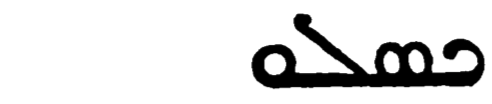
\includegraphics[height=10pt]{tables/099/03} } &
 Caslew &
 \textgreek{ἀπελλαῖος[?]} &
 3
\\
\midrule
 4 &
 \parbox[c]{5em}{
\includegraphics[height=10pt]{tables/099/04} } &
 Tebeth &
 \textgreek{αὐδυναῖος[?]} &
 5
\\
 5 &
 \parbox[c]{5em}{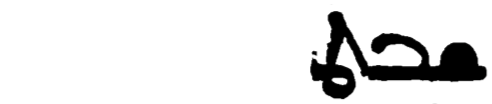
\includegraphics[height=10pt]{tables/099/05} } &
 Scebat &
 \textgreek{περίτιος[?]} &
 6
\\
 6 &
 \parbox[c]{5em}{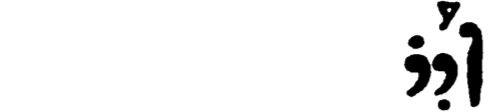
\includegraphics[height=10pt]{tables/099/06} } &
 Adar &
 \textgreek{δῦστρος[?]} &
 1
\\
\midrule
 7 &
 \parbox[c]{5em}{
\includegraphics[height=10pt]{tables/099/07} } &
 Nisan &
 \textgreek{ξανθικός[?]} &
 2
\\
 8 &
 \parbox[c]{5em}{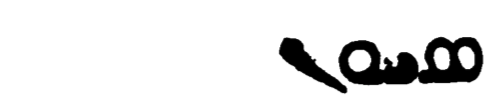
\includegraphics[height=10pt]{tables/099/08} } &
 Siwan &
 \textgreek{ἀρτεμίσιος[?]} &
 4
\\
 9 &
 \parbox[c]{5em}{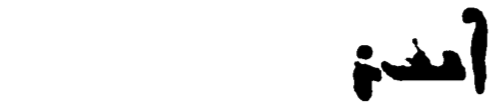
\includegraphics[height=10pt]{tables/099/09} } &
 Iijar &
 \textgreek{δαίσιος[?]} &
 5
\\
\midrule
 10 &
 \parbox[c]{5em}{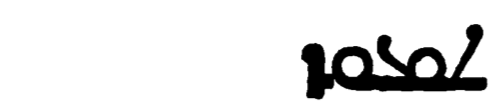
\includegraphics[height=10pt]{tables/099/10} } &
 Thamuz &
 \textgreek{πάνεμος[?]} &
 7
\\
 11 &
 \parbox[c]{5em}{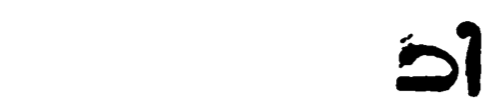
\includegraphics[height=10pt]{tables/099/11} } &
 Ab &
 \textgreek{λῶιος[?]} &
 1
\\
 12 &
% \parbox[c]{5em}{\includegraphics[height=\baselineskip]{tables/img/099_12} } &
% \includegraphics[height=\baselineskip]{tables/img/099_12} &
% \includegraphics[height=10pt]{tables/img/099_12} &
 \parbox[c]{5em}{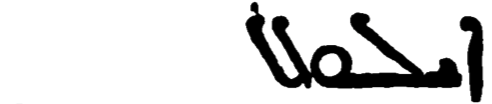
\includegraphics[height=10pt]{tables/099/12} } &
% \raisebox{-0.5\totalheight}{\includegraphics[height=10pt]{tables/img/099_12} } &
 Elul &
 \textgreek{γορπιαῖος[?]} &
 3
\\
 &
% \parbox[c]{5em}{\includegraphics[height=\baselineskip]{tables/img/099_13} } &
% \includegraphics[width=5em]{tables/img/099_13} &
% \includegraphics[height=10pt]{tables/img/099_13} &
 \parbox[c]{5em}{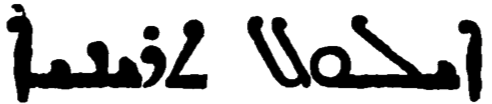
\includegraphics[height=10pt]{tables/099/13} } &
 Elul alter. &
 \textgreek{γορπιαῖος δευτερος.[?]} &
 5
\\
\bottomrule
\end{tabular}
%
\end{table}

\lipsum[31]
\begin{table}[htbp]
  %%% Liber II p101, PDF 184
%%
%% Table in the section "De periodo Chaldaeorum Alexandrea"
%% Title is given in the original.
%% The body of the table is filled mostly with Arabic, Turkish, Persian and
%% "Chatai", which all look arabic. There is also a column of Syrian,
%% same as what is seen in the table on p99.
%%
%% In the 1593 edition, p78, the body of this table is filled with Hebrew,
%% and the column of numbers is headed "Anni Schaichun."
%%
%% There is currently (nov 2017) no information on the Chaldean calendar
%% on Wikipedia
%%
%%% Count out columns for fixed-width source font
% 000000011111111112222222222333333333344444444445555555555666666666677777777778
% 345678901234567890123456789012345678901234567890123456789012345678901234567890
%
%% Select a general font size (uncomment one from the list)
%\tiny
%\scriptsize
%\footnotesize
%\small
\normalsize
%
%% Center the whole table left-right
\centering
%
%% Modify separation between columns
%\setlength{\tabcolsep}{1.6pt}
%
%% Modify distance between rows
%\renewcommand{\arraystretch}{1.3}
%%
\begin{tabular}{@{}l c r r r r r@{}}
\toprule
 \multicolumn{7}{c}{\Large\textsc{Nomina annorum Schaichun}}\\
 \multicolumn{7}{c}{\large\textsc{sive dodecaeteidos Chaldaicae}}
\\
\toprule
 \multicolumn{6}{c}{~} &
 \multicolumn{1}{c}{Chatai}
\\
 \multicolumn{1}{l}{Latini} &
 &
 \multicolumn{1}{c}{Syri} &
 \multicolumn{1}{c}{Arabes} &
 \multicolumn{1}{c}{Turcae} &
 \multicolumn{1}{c}{Persae} &
 \multicolumn{1}{c}{\& Ieguraei}
\\
\midrule
 \textsc{mus} &
 \rnum{i} &
 [?] &
 \textarabic{شيخون}[?] &
 \textarabic{شيخون}[?] &
 \textarabic{شيخون}[?] &
 \textarabic{شيخون}[?]
\\
 \textsc{taurus} &
 \rnum{ii} &
 [?] &
 \textarabic{شيخون}[?] &
 \textarabic{شيخون}[?] &
 \textarabic{شيخون}[?] &
 \textarabic{شيخون}[?]
\\
 \textsc{pardus} &
 \rnum{iii} &
 [?] &
 \textarabic{شيخون}[?] &
 \textarabic{شيخون}[?] &
 \textarabic{شيخون}[?] &
 \textarabic{شيخون}[?]
\\
\midrule
 \textsc{lepus} &
 \rnum{iiii} &
 [?] &
 \textarabic{شيخون}[?] &
 \textarabic{شيخون}[?] &
 \textarabic{شيخون}[?] &
 \textarabic{شيخون}[?]
\\
 \textsc{draco} &
 \rnum{v} &
 [?] &
 \textarabic{شيخون}[?] &
 \textarabic{شيخون}[?] &
 \textarabic{شيخون}[?] &
 \textarabic{شيخون}[?]
\\
 \textsc{serpens} &
 \rnum{vi} &
 [?] &
 \textarabic{شيخون}[?] &
 \textarabic{شيخون}[?] &
 \textarabic{شيخون}[?] &
 \textarabic{شيخون}[?]
\\
\midrule
 \textsc{equus} &
 \rnum{vii} &
 [?] &
 \textarabic{شيخون}[?] &
 \textarabic{شيخون}[?] &
 \textarabic{شيخون}[?] &
 \textarabic{شيخون}[?]
\\
 \textsc{ovis} &
 \rnum{viii} &
 [?] &
 \textarabic{شيخون}[?] &
 \textarabic{شيخون}[?] &
 \textarabic{شيخون}[?] &
 \textarabic{شيخون}[?]
\\
 \textsc{simia} &
 \rnum{ix} &
 [?] &
 \textarabic{شيخون}[?] &
 \textarabic{شيخون}[?] &
 \textarabic{شيخون}[?] &
 \textarabic{شيخون}[?]
\\
\midrule
 \textsc{gallina} &
 \rnum{x} &
 [?] &
 \textarabic{شيخون}[?] &
 \textarabic{شيخون}[?] &
 \textarabic{شيخون}[?] &
 \textarabic{شيخون}[?]
\\
 \textsc{canis} &
 \rnum{xi} &
 [?] &
 \textarabic{شيخون}[?] &
 \textarabic{شيخون}[?] &
 \textarabic{شيخون}[?] &
 \textarabic{شيخون}[?]
\\
 \textsc{porcus} &
 \rnum{xii} &
 [?] &
 \textarabic{شيخون}[?] &
 \textarabic{شيخون}[?] &
 \textarabic{شيخون}[?] &
 \textarabic{شيخون}[?]
\\
\bottomrule
\end{tabular}
%
\caption{Nomina annorum Schaichun}
\label{tab:101}

\end{table}

\lipsum[32]
\begin{table}[htbp]
  %%% Liber II p101, PDF 184
%%
%% Table in the section "De periodo Chaldaeorum Alexandrea"
%% Title is given in the original.
%% The body of the table is filled mostly with Arabic, Turkish, Persian and
%% "Chatai", which all look arabic. There is also a column of Syrian,
%% same as what is seen in the table on p99.
%%
%% In the 1593 edition, p78, the body of this table is filled with Hebrew,
%% and the column of numbers is headed "Anni Schaichun."
%%
%% There is currently (nov 2017) no information on the Chaldean calendar
%% on Wikipedia
%%
%%% Count out columns for fixed-width source font
% 000000011111111112222222222333333333344444444445555555555666666666677777777778
% 345678901234567890123456789012345678901234567890123456789012345678901234567890
%
%% Select a general font size (uncomment one from the list)
%\tiny
%\scriptsize
%\footnotesize
%\small
\normalsize
%
%% Center the whole table left-right
\centering
%
%% Modify separation between columns
%\setlength{\tabcolsep}{1.6pt}
%
%% Modify distance between rows
%\renewcommand{\arraystretch}{1.3}
%%
\begin{tabular}{@{}l c c c c c c@{}}
\toprule
 \multicolumn{7}{c}{\Large\textsc{Tabula characterismi}}\\
 \multicolumn{7}{c}{\large\textsc{mensium Iudaicorum}}
\\
\toprule
 
 ~ &
 \multicolumn{3}{c}{Communis} &
 \multicolumn{3}{c}{Embolimaeus}
\\
\cmidrule(lr){2-4}
\cmidrule(lr){5-7} 
 ~ &
 \multicolumn{1}{c}{\scriptsize Defectivus} &
 \multicolumn{1}{c}{\scriptsize Ordinarius} &
 \multicolumn{1}{c}{\scriptsize Abundans} &
 \multicolumn{1}{c}{\scriptsize Defectivus} &
 \multicolumn{1}{c}{\scriptsize Ordinarius} &
 \multicolumn{1}{c}{\scriptsize Abundans}
\\
\midrule
 \textsc{Tisri} &
 0 &
 0 &
 0 &
 0 &
 0 &
 0
 \\
 \textsc{Marcheswan} &
 2 &
 2 &
 2 &
 2 &
 2 &
 2
\\
 \textsc{Chaslev} &
 3 &
 3 &
 4 &
 3 &
 3 &
 4
\\
\midrule
 \textsc{Tebeth} &
 4 &
 5 &
 6 &
 4 &
 5 &
 6
\\
 \textsc{Schebat} &
 5 &
 6 &
 7 &
 5 &
 6 &
 7
\\
 \textsc{Adar prior.} &
 0 &
 0 &
 0 &
 7 &
 1 &
 2
\\
 \textsc{Adar poste.} &
 7 &
 1 &
 2 &
 2 &
 3 &
 4
\\
\midrule
 \textsc{Nisan} &
 1 &
 2 &
 3 &
 3 &
 4 &
 5
\\
 \textsc{Iiar} &
 3 &
 4 &
 5 &
 5 &
 6 &
 7
\\
 \textsc{Siwan} &
 4 &
 5 &
 6 &
 6 &
 7 &
 1
\\
\midrule
 \textsc{Thamuz} &
 6 &
 7 &
 1 &
 1 &
 2 &
 3
\\
 \textsc{Ab} &
 7 &
 1 &
 2 &
 2 &
 3 &
 4
\\
 \textsc{Elul} &
 2 &
 3 &
 4 &
 4 &
 5 &
 6
\\
\bottomrule
\end{tabular}
%
\end{table}

\lipsum[33]
\begin{table}[htbp]
  %%% Liber II p109, PDF 192
%%
%% Table in the section "De periodo Hipparchi et vero anno lunari"
%% No title is given in the original.
%%
%%% Count out columns for fixed-width source font
% 000000011111111112222222222333333333344444444445555555555666666666677777777778
% 345678901234567890123456789012345678901234567890123456789012345678901234567890
%
%% Select a general font size (uncomment one from the list)
%\tiny
%\scriptsize
%\footnotesize
%\small
\normalsize
%
%% Center the whole table left-right
\centering
%
%% Modify separation between columns
%\setlength{\tabcolsep}{1.6pt}
%
%% Modify distance between rows
%\renewcommand{\arraystretch}{1.3}
%%
\begin{tabular}{@{}r r r r r @{}}
\toprule
 \multicolumn{2}{c}{Cycli Hyparchi} &
 \multicolumn{2}{c}{Cycli Calippi} &
 \multicolumn{1}{c}{Cycli Metonis}
\\
\cmidrule(lr){1-2}
\cmidrule(lr){3-4}
\cmidrule(lr){5-5}
 \multicolumn{1}{c}{\scriptsize Dies collecti} &
 \multicolumn{1}{c}{\scriptsize Scrupula} &
 \multicolumn{1}{c}{\scriptsize Dies collecti} &
 \multicolumn{1}{c}{\scriptsize Scrupula} &
 \multicolumn{1}{c}{\scriptsize Dies collecti} 
\\
 ~ & 16
\\
\midrule
 6939 &
 11 &
 6939 &
 45 &
 6940
\\
 13879 &
 6 &
 13879 &
 30 &
 13880
\\
 20819 &
 1 &
 20819 &
 15 &
 20820
\\
 27758 &
 12 &
 27759 &
 0 &
 27760
\\
\midrule
 34698 &
 7 &
 34698 &
 45 &
 34700
\\
 41638 &
 2 &
 41638 &
 30 &
 41640
\\
 41577 &
 13 &
 48578 &
 15 &
 48580
\\
 55517 &
 8 &
 55518 &
 0 &
 55320
\\
\midrule
 62457 &
 3 &
 62457 &
 45 &
 62460
\\
 69396 &
 14 &
 69397 &
 30 &
 69400
\\
 76336 &
 9 &
 76337 &
 15 &
 76340
\\
 83276 &
 4 &
 83277 &
 0 &
 83280
\\
\midrule
 90215 &
 15 &
 90216 &
 45 &
 90220
\\
 97155 &
 10 &
 97156 &
 30 &
 97160
\\
 104095 &
 5 &
 104096 &
 15 &
 104100
\\
 111035 &
 0 &
 111036 &
 0 &
 111040
\\
\bottomrule
\end{tabular}
%
\caption{Cycli Hyparchi, Calippi et Metonis}
\label{tab:p109}

\end{table}

\lipsum[34]
\begin{table}[htbp]
  %%% Liber II p110, PDF 193
%%
%% Table in the section "De periodo Arabum Hagarenorum"
%% No title is given in the original.
%% The second column is in Arabic
%% Modern names of the months as given on the "Islamic calendar" page of
%% Wikipedia were used to fill this column. The English transcriptions 
%% given there are added here as comments.
%%
%%% Count out columns for fixed-width source font
% 000000011111111112222222222333333333344444444445555555555666666666677777777778
% 345678901234567890123456789012345678901234567890123456789012345678901234567890
%
%% Select a general font size (uncomment one from the list)
%\tiny
%\scriptsize
%\footnotesize
%\small
\normalsize
%
%% Center the whole table left-right
\centering
%
%% Modify separation between columns
%\setlength{\tabcolsep}{1.6pt}
%
%% Modify distance between rows
%\renewcommand{\arraystretch}{1.3}
%%
\begin{tabular}{@{}r r l@{}}
\toprule
 0 &
 % Rabī‘ al-awwal (the first spring)
 \textarabic{رَبيع الأوّل}[?] &
 \emph{Rabiu prior}
\\
 2 &
 % Rabī‘ ath-thānī (the second spring)
 \textarabic{رَبيع الثاني}[?] &
 \emph{Rabiu posterior}
\\
 3 &
 % Jumādá al-ūlá (the first of parched land)
 \textarabic{جُمادى الأولى}[?] &
 \emph{Giumediiu prior}
\\
\midrule
 5 &
 % Jumādá al-ākhirah (the last of parched land)
 \textarabic{جُمادى الآخرة}[?] &
 \emph{Giumediiu posterior}
\\
 6 &
 % Rajab (respect, honour)
 \textarabic{رَجَب}[?] &
 \emph{Regebu}
\\
 1 &
 % Sha‘bān (scattered)
 \textarabic{شَعْبان}[?] &
 \emph{Saabenu}
\\
\midrule
 2 &
 % Ramaḍān (burning heat)
 \textarabic{رَمَضان}[?] &
 \emph{Ramadhanu}
\\
 4 &
 % Shawwāl (raised)
 \textarabic{شَوّال}[?] &
 \emph{Schevvalu}
\\
 5 &
 % Dhū al-Qa‘dah (the one of truce/sitting)
 \textarabic{ذو القعدة}[?] &
 \emph{Dulkaidathi}
\\
\midrule
 7 &
 % Dhū al-Ḥijjah (the one of pilgrimage)
 \textarabic{ذو الحجة}[?] &
 \emph{Dulhagaiathi}
\\
 1 &
 % Muḥarram (forbidden)
 \textarabic{مُحَرَّم}[?] &
 \emph{Muharramu}
\\
 3 &
 % Ṣafar (void)
 \textarabic{صَفَر}[?] &
 \emph{Tzepharu}
\\
\bottomrule
\end{tabular}
%
\caption{Periodo Hagarena}
%
\end{table}

%\begin{table}[htbp]
%  %%% Liber II p67, PDF 150
%%
%% Conversion of Νεομηνιαι της Οκταετηριδος καθ´ εκαστον ετος
%% eliminating most of the Greek.
%% - The column headers (ἔτος προτον, etc) are simply year numbers
%% - The body of the table consists of Greek numbers for days, and the names
%%   of the months, which are also listed in the first columns.
%%   The numbers are converted to arabic numerals, and the names of the months
%%   are indexed with roman numerals, and a column of those roman numerals is
%%   added to the left of the column with the Greek names of the months.
%%
%%% Count out columns for fixed-width source font
% 000000011111111112222222222333333333344444444445555555555666666666677777777778
% 345678901234567890123456789012345678901234567890123456789012345678901234567890
%
%% Select a general font size (uncomment one from the list)
%\tiny
%\scriptsize
%\footnotesize
%\small
%\normalsize
%% Center the whole table left-right
\centering
%% Modify distance between rows
\renewcommand{\arraystretch}{1.2}
%% Modify separation between columns
\setlength{\tabcolsep}{2.0pt}
%
\begin{tabular}{@{}cl llllllll@{}}
\toprule
\multicolumn{2}{ c }{~} &
\multicolumn{8}{ c }{annum}
\\
\cmidrule{3-10}
\multicolumn{2}{ c }{Mensis lunaris} &
\multicolumn{1}{c}{1} &
\multicolumn{1}{c}{2} &
\multicolumn{1}{c}{3} &
\multicolumn{1}{c}{4} &
\multicolumn{1}{c}{5} &
\multicolumn{1}{c}{6} &
\multicolumn{1}{c}{7} &
\multicolumn{1}{c}{8}
\\
\midrule
\textsc{vii} & \textgreek{γαμηλιών} &
 1.\textsc{vii} &
25.\textsc{vi} &
18.\textsc{vi} &
 8.\textsc{vii} &
 1.\textsc{vii} &
26.\textsc{vi} &
16.\textsc{vii} &
 8.\textsc{vii}
\\
\textsc{viii} & \textgreek{ανθεστηριών} &
 1.\textsc{viii} &
23.\textsc{vii} &
15.\textsc{vii} &
 8.\textsc{viii} &
 1.\textsc{viii} &
23.\textsc{vii} &
15.\textsc{viii} &
 8.\textsc{viii}
\\
\textsc{ix} & \textgreek{ἐλαφηβολιών} &
 1.\textsc{ix} &
23.\textsc{viii} &
15.\textsc{viii} &
 7.\textsc{ix} &
30.\textsc{viii} &
23.\textsc{viii} &
15.\textsc{ix} &
 7.\textsc{ix}
\\
\midrule
\textsc{x} & \textgreek{μυονυχιών} &
30.\textsc{ix} &
22.\textsc{ix} &
14.\textsc{ix} &
 7.\textsc{x} &
30.\textsc{ix} &
22.\textsc{ix} &
14.\textsc{x} &
 7.\textsc{x}
\\
\textsc{xi} & \textgreek{θαργηλιών} &
30.\textsc{x} &
22.\textsc{x} &
14.\textsc{x} &
 6.\textsc{xi} &
29.\textsc{x} &
22.\textsc{x} &
14.\textsc{xi} &
 6.\textsc{xi}
\\
\textsc{xii} & \textgreek{σκιῤῥοφοριών} &
29.\textsc{xi} &
21.\textsc{xi} &
14.\textsc{xi} &
 6.\textsc{xii} &
24.\textsc{xi} &
21.\textsc{xi} &
13.\textsc{xii} &
 6.\textsc{xii}
\\
\midrule
\textsc{i} & \textgreek{ἑκατομβαιών} &
29.\textsc{xii} &
21.\textsc{xii} &
13.\textsc{xii} &
 6.\textsc{i} &
29.\textsc{xii} &
21.\textsc{xii} &
13.\textsc{i} &
 5.\textsc{i}
\\
\textsc{ii} & \textgreek{μεταγειτνιών} &
28.\textsc{i} &
20.\textsc{i} &
13.\textsc{i} &
 5.\textsc{ii} &
28.\textsc{i} &
20.\textsc{i} &
12.\textsc{ii} &
 5.\textsc{ii}
\\
\textsc{iii} & \textgreek{βοηδρομιών} &
28.\textsc{ii} &
20.\textsc{ii} &
12.\textsc{ii} &
 5.\textsc{iii} &
28.\textsc{ii} &
20.\textsc{ii} &
12.\textsc{iii} &
 4.\textsc{iii}
\\
\midrule
\textsc{iv} & \textgreek{πυανεψιών} &
27.\textsc{iii} &
19.\textsc{iii} &
12.\textsc{iii} &
 5.\textsc{iv} &
27.\textsc{iii} &
20.\textsc{iii} &
11.\textsc{iv} &
 4.\textsc{iv}
\\
\textsc{v} & \textgreek{μαιμακτηριών} &
27.\textsc{iv} &
19.\textsc{iv} &
11.\textsc{iv} &
 4.\textsc{v} &
27.\textsc{iv} &
19.\textsc{iv} &
11.\textsc{v} &
 3.\textsc{v}
\\
\textsc{vi} & \textgreek{ποσειδεών} $\overline{\alpha}$&
26.\textsc{v} &
18.\textsc{v} &
11.\textsc{v} &
 3.\textsc{vi} &
26.\textsc{v} &
19.\textsc{v} &
11.\textsc{vi} &
 3.\textsc{vi}
\\
\textsc{vi} & \textgreek{ποσειδεών} $\overline{\beta}$&
26.\textsc{vi} $\overline{\alpha}$ &
    \multicolumn{1}{c}{$\circ$} &
10.\textsc{vi} &
    \multicolumn{1}{c}{$\circ$} &
    \multicolumn{1}{c}{$\circ$} &
18.\textsc{vi} &
    \multicolumn{1}{c}{$\circ$} &
\multicolumn{1}{c}{~}\\
\bottomrule
\end{tabular}
%
\caption{Neomeniae octaeteridai Harpali per annum}

%\end{table}

\lipsum[40]


\listoftables
\end{document}
